%%%%%%%%%%%%%%%%%%%%%%%%%%%%%%%%%%%%%%%%%%%%%%%%%%%%%%%%%%%%%%%%%%%%%%%%%%%%%%
%% Paying for Your Own Data:
%% A Closed-Loop Benchmark for Scientific ML Agents
%%
%% Target venue: NeurIPS Datasets & Benchmarks Track.
%% Compile with pdfLaTeX + BibTeX (Overleaf's default recipe works as-is).
%% See README.md for the fill-in workflow and for how to retarget the venue.
%%%%%%%%%%%%%%%%%%%%%%%%%%%%%%%%%%%%%%%%%%%%%%%%%%%%%%%%%%%%%%%%%%%%%%%%%%%%%%

\documentclass{article}

% ---------------------------------------------------------------- venue ----
% Style options:
%   [eandd]            anonymous submission, line numbers on   <- for review
%   [preprint,eandd]   named authors, no line numbers          <- for arXiv
%   [final,eandd]      camera ready
% NOTE: for NeurIPS 2026 the Datasets & Benchmarks track is the "Evaluations
% and Datasets" track and its style option is [eandd]; [datasets] is not a
% declared option of neurips_2026.sty and will raise an error.
\usepackage[preprint,eandd]{neurips_2026}

% -------------------------------------------------------------- packages ---
\usepackage[utf8]{inputenc}
\usepackage[english]{babel}
\usepackage{amsmath,amssymb,amsfonts}
\usepackage{booktabs}
\usepackage{array}
\usepackage{multirow}
\usepackage{graphicx}
\usepackage{xcolor}
\usepackage{xspace}
\usepackage{microtype}
\usepackage{nicefrac}
\usepackage{enumitem}
\usepackage{caption}
\usepackage{url}
\usepackage[colorlinks=true,linkcolor=black,citecolor=black,urlcolor=blue!60!black]{hyperref}

\usepackage{tcolorbox}
\tcbuselibrary{skins,breakable}

\usepackage{tikz}
\usetikzlibrary{positioning,arrows.meta,shapes.geometric,calc,fit,backgrounds}

% Float placement only -- the text block, margins and font sizes are exactly as
% the venue style sets them; these parameters just let LaTeX put more text on a
% page that already carries a float, instead of leaving it half empty.
\renewcommand{\topfraction}{0.92}
\renewcommand{\bottomfraction}{0.85}
\renewcommand{\textfraction}{0.06}
\renewcommand{\floatpagefraction}{0.8}
\setcounter{topnumber}{3}
\setcounter{totalnumber}{4}

\captionsetup{font=small,labelfont=bf,skip=6pt}
\setlist{nosep,leftmargin=1.4em}

%%%%%%%%%%%%%%%%%%%%%%%%%%%%%%%%%%%%%%%%%%%%%%%%%%%%%%%%%%%%%%%%%%%%%%%%%%%%%%
%% macros.tex -- notation shortcuts and the open-slot ("FILL") machinery
%%%%%%%%%%%%%%%%%%%%%%%%%%%%%%%%%%%%%%%%%%%%%%%%%%%%%%%%%%%%%%%%%%%%%%%%%%%%%%

%%%%%%%%%%%%%%%%%%%%%%%%%%%%%%%%%%%%%%%%%%%%%%%%%%%%%%%%%%%% open slots %%%%%
%
% Every number that depends on the running campaign is marked with \FILL or
% \FILLBOX. Both are listed, with page numbers, by \listoffills at the end of
% the document.
%
% Set \showfillfalse (below) to make every marker vanish from the PDF --
% useful for checking page count against the venue limit, since the markers
% themselves consume space.

\newif\ifshowfill
\showfilltrue          % <-- flip to \showfillfalse for a clean, marker-free PDF

\definecolor{fillbg}{HTML}{FFF3CD}
\definecolor{fillrule}{HTML}{D39E00}
\definecolor{filltext}{HTML}{7A5C00}

% Record every slot into the .fil auxiliary file so \listoffills can print it.
\newcommand{\recordfill}[1]{%
  \addcontentsline{fil}{figure}{\protect\numberline{}\small #1}%
}

% --- inline slot: \FILL{what is missing} ------------------------------------
% The tag is boxed (short, never needs to break); the text is plain coloured
% prose so it wraps normally. Do not put the text inside \colorbox -- an
% unbreakable box produces enormous overfull lines.
\newcommand{\FILL}[1]{%
  \recordfill{#1}%
  \ifshowfill
    \colorbox{fillbg}{\textcolor{filltext}{\scriptsize\textsf{\bfseries FILL}}}%
    \,\textcolor{filltext}{\small #1}%
  \fi
}

% --- paragraph-level slot: \begin{FILLBOX} ... \end{FILLBOX} ----------------
\newenvironment{FILLBOX}[1][open slot]{%
  \recordfill{#1}%
  \ifshowfill
    \begin{tcolorbox}[
      breakable, enhanced, sharp corners,
      colback=fillbg, colframe=fillrule, boxrule=0.4pt,
      left=5pt, right=5pt, top=4pt, bottom=4pt,
      before skip=6pt, after skip=6pt,
      fontupper=\small\color{filltext}]%
    \textsf{\bfseries [FILL]}\ \ignorespaces
  \else
    \setbox0\vbox\bgroup
  \fi
}{%
  \ifshowfill
    \end{tcolorbox}%
  \else
    \egroup
  \fi
}

% --- the index of open slots -------------------------------------------------
\makeatletter
\newcommand{\listoffills}{%
  \section*{Open slots in this draft}%
  \small
  \@starttoc{fil}%
}
\makeatother

% Placeholder for a number not yet measured, inside tables and running text.
\newcommand{\tbd}{\textcolor{fillrule}{\textbf{--}}}

%%%%%%%%%%%%%%%%%%%%%%%%%%%%%%%%%%%%%%%%%%%%%%%%%%%%%%%%%%%%%%% notation %%%%

\newcommand{\psifield}{\psi}
\newcommand{\Rgrid}{R}
\newcommand{\Zgrid}{Z}
\newcommand{\relltwo}{\mathrm{relL2}}
\newcommand{\Ip}{I_{\mathrm{p}}}
\newcommand{\rzero}{r_{0}}
\newcommand{\gs}{Grad--Shafranov}
\newcommand{\GS}{Grad--Shafranov}

% levels and harnesses, so they are typeset consistently everywhere
\newcommand{\Lzero}{\textsf{L0}}
\newcommand{\Lone}{\textsf{L1}}
\newcommand{\Ltwo}{\textsf{L2}}
\newcommand{\Lthree}{\textsf{L3}}
\newcommand{\hn}[1]{\textsf{#1}}

% code-ish inline
\newcommand{\code}[1]{\texttt{\small #1}}

\newcommand{\eg}{e.g.\xspace}
\newcommand{\ie}{i.e.\xspace}


% ---------------------------------------------------------------- title ----
\title{Paying for Your Own Data:\\A Closed-Loop Benchmark for Scientific ML Agents}

\author{%
  Hindy Ros \\
  Massachusetts Institute of Technology \\
  \texttt{hindyros@mit.edu} \\
  \And
  Deepjyoti Deka \\
  MIT Energy Initiative \\
  Massachusetts Institute of Technology \\
  \texttt{deepj87@mit.edu} \\
}

\begin{document}
\maketitle

\begin{abstract}
Benchmarks for coding and machine-learning agents overwhelmingly hand the agent
its data. We present a benchmark in which the agent must \emph{generate its own
data from an expensive physics simulator under a fixed solve budget}, then ship
a predictor that is scored independently on a frozen grid it never sees. The
task is surrogate modelling of the \GS{} plasma equilibrium: an agent must learn
to drive a finite-element solver, design a sampling campaign (an initial
space-filling design plus up to three adaptive rounds of exactly 100 solves),
train a surrogate mapping five shaping parameters to a $96\times64$
poloidal-flux field, and evaluate itself honestly. Every condition emits the
same machine-checkable contract, so any agent substrate is scored identically.
We evaluate four agent harnesses at two access levels---library-assisted
(\Ltwo{}, may import a proven pipeline library) and from-scratch (\Lthree{},
imports audited and forbidden)---with \emph{all cells on one model}, alongside
a zero-LLM scripted baseline running the same pipeline code at a matched solve
budget.
Across 59 runs, from-scratch agents beat library-assisted ones in \emph{all
four} substrates (median relative-$L_2$ $0.137$ vs $0.229$; stratified rank test
$z = -4.17$, permutation $p \approx 5\times10^{-5}$, blocked on harness). Our
central finding concerns \emph{verification}: \textbf{15 of 49 scored runs
passed every contract gate while being physically invalid}, a rate that is
substrate-specific ($11/20$ and $4/9$ for two harnesses, $0/20$ for the other
two) and independent of access level. Self-reported error diverges from
independently scored error by up to $0.93$, and large honesty gaps and invalid
artifacts are largely \emph{different} runs, so neither detects the other.
Machine-checkable deliverable contracts, the standard instrument in this
literature, detect none of this. We therefore separate three questions a
benchmark must ask---did the agent deliver, is the artifact physically valid,
and did it tell the truth---and measure all three, alongside a deterministic
LLM-free account of the method chain each agent actually built.
\end{abstract}

\section{Introduction}
\label{sec:intro}

Agentic machine-learning benchmarks have converged on a shape: present the agent
with a dataset and a metric, and see how good a model it can fit. MLE-bench
draws on Kaggle competitions; MLAgentBench, DSBench, ScienceAgentBench and
related suites vary the domain and the scaffolding but keep the
shape.\footnote{Citations are collected in Section~\ref{sec:related}.} The data
exists before the agent starts.

Real computational science does not look like that. The expensive step is
usually \emph{acquiring} the data---running the simulation, the experiment, the
solve---and the interesting decision is \emph{where to spend the next unit of
budget}. An agent good at fitting a given dataset may be useless at deciding
which equilibria are worth computing. This benchmark restores that decision: the
agent is given a solver, a parameter space and a budget, and must decide what to
compute (Figure~\ref{fig:loop}, Appendix~\ref{app:loop}).

The ground-truth operator is TokaMaker (Open FUSION Toolkit), a finite-element
solver for the axisymmetric \GS{} equation
$\Delta^{*}\psi = -\mu_{0}R^{2}p'(\psi) - F(\psi)F'(\psi)$ on a triangular mesh
of a D-shaped plasma cross-section. It is a good instrument here because it is
expensive and \emph{failable}, so the feasible set must be discovered rather
than assumed; high-dimensional in the output (a $96\times64$ flux field, NaN
outside the plasma boundary) but low-dimensional in the input, making
dimensionality reduction a real design decision; unforgiving about physics,
since flux is signed and physical and an agent that quietly clips or
renormalises produces a field that looks plausible and is wrong; and not
memorisable.

\paragraph{Contributions.}
\textbf{(i) A closed-loop scientific-ML benchmark} in which the agent pays for
its own data from an expensive solver under a fixed budget, with a
machine-checkable deliverable contract, independent scoring on a frozen grid,
and a graded scaffolding ladder from a zero-LLM scripted policy to from-scratch,
all rungs inside the identical contract (Section~\ref{sec:benchmark}).
\textbf{(ii) A model-controlled harness comparison}---four substrates on one
identical model, so ``which agent framework'' is not confounded with ``which
model'', a confound we found in our own earlier campaigns---which finds that
library access makes agents \emph{worse} in all four
(Section~\ref{sec:results}).
\textbf{(iii) A verification layer} distinguishing delivery, physical validity
and self-report honesty, which finds that 31\% of scored runs pass every
contract gate while being physically invalid
(Section~\ref{sec:verification}).
\textbf{(iv) A deterministic, LLM-free account of what each agent built}---its
chain of methods, its per-round decision logic, and whether its code agrees with
its own prose---which is what makes the level effect interpretable
(Section~\ref{sec:agentlogic}).

\section{Related work}
\label{sec:related}

\paragraph{Agentic coding, ML-engineering and scientific-agent benchmarks.}
The dominant evaluation shape gives the agent a repository or a dataset and
scores the artifact it produces---SWE-bench \citep{jimenez2024swebench},
AgentBench \citep{liu2024agentbench}, and, closest to us, the ML-engineering
suites: MLE-bench \citep{chan2024mlebench} on Kaggle competitions graded against
the private leaderboard, MLAgentBench \citep{huang2024mlagentbench} on iterative
experimentation over fixed datasets, DSBench \citep{jing2024dsbench} on
data-science competitions. A second line targets science: ScienceAgentBench
\citep{chen2025scienceagentbench}, DiscoveryBench
\citep{majumder2025discoverybench} and BixBench \citep{mitchener2025bixbench}
over provided datasets, CORE-Bench \citep{siegel2024corebench} on computational
reproducibility, PaperBench \citep{starace2025paperbench} on replicating ML
papers, RE-Bench \citep{wijk2024rebench} against human experts on open-ended
research engineering. In all of them the training data is supplied in advance
and is identical for every agent---exactly what makes them clean comparisons,
and what removes acquisition from the decisions being measured.

\paragraph{What we add.}
The gap is not that no one acquires data---active learning
\citep{settles2009active}, Bayesian experimental design
\citep{chaloner1995bayesian} and space-filling designs \citep{mckay1979lhs}
supply the strategies a competent agent might reach for, and the baseline it
must beat. It is that \emph{agentic coding benchmarks do not make the
acquisition policy part of what is scored}. To our knowledge, as of mid-2026, no
existing agent benchmark requires the agent to (i) drive an expensive,
failure-prone numerical solver it has not been handed a working harness for,
(ii) allocate a hard budget across adaptive rounds, and (iii) be scored on a
frozen set it never sees, with a zero-LLM scripted policy running inside the
identical contract as the reference point. Two recent works come closest:
AstaBench \citep{bragg2025astabench} assembles a large scientific-agent suite,
motivated by the same complaint about confounders that motivates our model
control, but supplies the tools and data rather than scoring acquisition; and a
position paper argues that the execution harness, not the model it wraps, is
often the binding constraint on agent performance \citep{zhang2026harness},
of which our campaign is a direct empirical test
(Section~\ref{sec:harness-effect}).

\paragraph{Agent substrates.}
The harnesses we compare are existing systems, not contributions of this paper:
URSA \citep{ursa2025}, a planner/executor pair built on LangGraph, part of the
LangChain project \citep{langchain2022}; DSPy \citep{khattab2024dspy}, whose
typed modules we also use for the \Lone{} decision layer and whose GEPA
optimiser \citep{agrawal2025gepa} we use for prompt optimisation; and two
commercial CLI coding agents, evaluated as we found them.

\section{The benchmark}
\label{sec:benchmark}

\subsection{The task, the contract, and the scoring}
\label{sec:task}

The agent receives a frozen, versioned problem statement
(Appendix~\ref{app:tasktext}) giving: the forward problem---fixed-boundary
equilibria of D-shaped plasmas in five parameters ($\rzero$, $a$, $\kappa$,
$\delta$, $\Ip$) over stated ranges at the solver's default profiles; a campaign
structure with a hard budget---at most 150 initial space-filling solves then up
to three adaptive rounds of exactly 100 new solves each, failures included, with
each round's points required to be chosen from the current model or data, so a
one-shot design is explicitly insufficient; a stopping criterion---stop early
once validation error reaches $\le 0.30\times$ the mean-predictor baseline, on a
validation set kept separate from the test set; a held-out test set of at least
20 solves at a recorded seed, never used for training, selection or acquisition;
and a requirement to report whether the adaptive sampling actually helped, ``or
an honest statement that it did not''. Four process gates are mandatory and
identical for every condition: a \emph{meshing milestone}, a \emph{pilot gate}
($\ge 20$ solves at $\ge 50\%$ success before the rounds begin), a
\emph{storage-validation gate} (a solve counts only after its stored artifact is
re-read from disk and confirmed finite), and a \emph{deliverable self-test} (run
every documented command in a fresh process before declaring done).

\paragraph{The deliverable contract.}
Every condition emits the same artifacts, checked mechanically. The nine checks
(Appendix~\ref{app:gates}) require the three artifacts to exist and be
non-empty, \code{report.json} to parse and carry the required keys,
\code{predict.py} to run to completion as a subprocess on sample parameters,
and its output to have the right shape on the right grid. One
further gate applies at \Lthree{} only---a static audit that no workspace file
imports the platform library---so \Lthree{} runs face nine gates and \Ltwo{}
eight. \code{contract.passed} is the flat \textsc{and} of them: no weighting, no
partial credit. The scoring subprocess is stripped of provider credentials, so
\code{predict.py} must work offline, and runs in its own process group so a
timeout reaps the solver's children. Critically, \code{report\_keys}
\textbf{checks key \emph{presence}, never correctness}: self-reported metrics
are recorded verbatim and never cross-checked, which is what makes the honesty
measurement of Section~\ref{sec:honesty} possible.

\paragraph{Independent scoring.}
Predictions are scored against a frozen test set of 60 parameter vectors (seed
\code{20260809}, all 60 converged) solved once and stamped with provenance---
solver version, the SHA-256 of both the parameter file and the grid, and a
scoring epoch---so a score is only ever pooled with scores computed the same
way. The archive is never regenerated. The metric is per-sample relative $L_2$
over the finite ground-truth points, and \textbf{a NaN prediction at a finite
ground-truth point is scored as a full-magnitude miss}, never skipped, since
otherwise an all-NaN prediction would score as perfect
(Appendix~\ref{app:scoring}). Accuracy is quoted against the trivial
mean-flux-map predictor on the same set, which scores $0.4933$.

\subsection{The access-level ladder, and the substrates}
\label{sec:ladder}

Four levels, all emitting the identical contract and scored on the identical
frozen set: \Lzero{} \emph{scripted}, the pre-written pipeline with seeded
heuristic decisions and zero LLM calls; \Lone{} \emph{structured}, the same
pipeline with an LLM making only typed decisions; \Ltwo{}
\emph{library-assisted}, where the agent writes the glue code and may import the
platform library; and \Lthree{} \emph{from-scratch}, where it writes everything
and the import is forbidden and audited. \Lzero{} is the golden baseline---same
seed, same decisions, no model---and having a zero-LLM condition scored on the
same frozen set is what lets us say how much of a score is the task and how much
is the agent. Four agent substrates implement one adapter each behind the same
interface: \hn{ursa} (a plan/execute agent pair on LangGraph), \hn{dspy} (plan
$\rightarrow$ per-step ReAct $\rightarrow$ review $\rightarrow$ fix), and
\hn{pi} and \hn{cursor} (CLI coding agents); adding a substrate is one adapter
module and one registry entry.

\paragraph{Is the task hard for the right reasons?}
\label{sec:characterisation}
Three facts from a direct sweep independent of any agent, detailed in
Appendix~\ref{app:characterisation}. The \emph{best model family changes with
$N$}---polynomial ridge up to $N = 200$, kernel ridge from $400$---so model
selection depends on the data the agent chose, and the 450-solve bound sits
where that still matters. At matched budget space-filling beats uniform-random
by $21\%$ at $N = 100$ and $6\%$ by $1600$, while clustered sampling is
catastrophic everywhere. And the surrogate \emph{collapses out of
distribution}---trained on half the parameter space and tested on the other,
ratio $0.94$ against $0.38$--$0.40$ within-distribution---so an agent that
samples badly does not lose a few percent; it produces a model that fails
completely off-distribution and, evaluating itself on its \emph{own} test set,
may never notice.

\section{Experimental design}
\label{sec:design}

\paragraph{Conditions and model control.}
$\{\Ltwo{}, \Lthree{}\} \times \{\hn{ursa}, \hn{dspy}, \hn{pi}, \hn{cursor}\}
= 8$ cells, replicated, plus a budget-matched \Lzero{} reference arm. We
attempted 59 runs and scored 49. Replicate counts are deliberately unequal---two
substrates at $n=10$ and two at $n=5$---because the campaign was budgeted in
dollars rather than in runs and one substrate costs an order of magnitude more
per run than another; failures reduce some cells further, and every denominator
in this paper counts attempts, not survivors. Every cell runs the \emph{same}
model, \code{gpt-5.2}, pinned per adapter inside the task specification because
the adapters disagree about how a model is named. Pinning it in the frozen task
text rather than as a command-line override is what makes the control auditable:
the model string is recorded three independent times per run. In our own earlier
campaign one harness ran a different model family from the others, making
``harness effect'' and ``model effect'' inseparable; a fifth adapter is excluded
here for the same reason, being unable to run the pinned model. Harness versions
were \hn{ursa} 0.15.1, \hn{dspy} 3.2.1, \hn{pi} 0.73.1 and \hn{cursor}
2026.09.18, against Open FUSION Toolkit 26.6---\textbf{recorded from the
machine, not from the run records}, which stamp the task hash, prompt version,
model and replicate index but not the substrate's version---a provenance gap in
our harness that we state rather than imply otherwise.

\paragraph{Equal compute budgets, and why they are hard to enforce.}
Giving every substrate the same budget was the hardest engineering requirement
in the benchmark. Two adapters accepted a \code{timeout\_seconds} argument and
silently ignored it; fixing that exposed two deeper failures---a timeout raised
as an ordinary exception is \emph{swallowed} by the broad \code{except Exception}
handlers agent frameworks wrap their step loops in, and, \code{signal.alarm}
being one-shot, one harness then ran over ten hours against a 90-minute cap; and
killing the agent does not stop the work, because a timing-out
\code{subprocess.run} waits again on pipes the solver's grandchildren hold open,
which left one cell deadlocked for 9\,h\,19\,m. The lesson generalises past this
benchmark---\textbf{an agent harness is third-party code and cannot be trusted
to honour a deadline from inside}---so we enforce the budget in-adapter, by
process-group kill, and by a driver watchdog nothing inside the cell can
intercept (Appendix~\ref{app:budget}). We also equalised \code{feedback\_rounds}
to 1, the only value all four adapters honour identically. Held fixed: prompt
text (version 3, hashed per run), the frozen grid, the 60-parameter test set,
the gate set and the scoring rule; the \Ltwo{} and \Lthree{} problem texts are
byte-identical except for ten hunks, all concerning access level
(Appendix~\ref{app:tasktext}).

\paragraph{Analysis, and one post-hoc change we must disclose.}
The unit of analysis is the cell. Pass rates carry \textbf{Wilson score
intervals} \citep{wilson1927probable}, which---unlike the normal
approximation---do not collapse to zero width at $0/n$ or $n/n$; relative-$L_2$
is summarised by \textbf{medians with percentile bootstrap intervals}
\citep{efron1979bootstrap}, not means, because a single catastrophic replicate
makes a mean uninterpretable and we have several. The \Ltwo{}/\Lthree{} contrast
is paired within harness, since harness is a blocking factor rather than a
treatment. We pre-specified an exact two-sided sign test over the four harness
pairs. That test cannot return a $p$ below $0.125$ at four pairs, and the
campaign produced a unanimous $4/4$ direction, so we \textbf{changed the primary
test after seeing the data} to a stratified rank statistic in the van Elteren
family \citep{vanelteren1960combination}, which uses all 49 scored runs while
still permuting labels only within harness. This is post-hoc and we treat it as
such: the analysis tool prints all three tests on every run, all three appear in
Section~\ref{sec:l2l3}, and the conclusion carries the caveat. Per-cell
orderings are exploratory throughout; the pooled level contrast is the claim
that carries weight.

\section{Results}
\label{sec:results}

The campaign ran 59 cells to completion or failure and scored 49, at a measured
cost of \$197.78;\footnote{From the directory-keyed cost report. The aggregate
tool reports \$199.76 because it joins on \code{run\_id}, which two substrates
reuse across sibling replicate directories; we report the former and note the
defect rather than silently choosing.} ten runs produced no score
(Section~\ref{sec:taxonomy}).

\begin{table}[tbp]
\centering
\caption{Per-cell results. $n$ counts \emph{attempts}, so a replicate killed
before writing a deliverable counts against the pass rate; \emph{sc.} counts
those with a frozen-set score. Relative $L_2$ is the median over scored
replicates with a percentile bootstrap interval (10\,000 resamples, seed
\code{20260917}) on the frozen 60-parameter test set, baseline $0.4933$;
``valid'' passes every gate \emph{and} the physical diagnostics of
Section~\ref{sec:validity}, the complement in every cell being a run that passed
every gate while physically invalid. The \Lzero{} row is the pipeline run
directly, so it emits no contract and its interval is the range over three
seeds. \hn{cursor} and \hn{ursa} costs are derived from token counts at a
committed price table, not vendor billing.}
\label{tab:main}
\footnotesize
\setlength{\tabcolsep}{4.5pt}
\begin{tabular}{@{}llrrcrcrr@{}}
\toprule
\textbf{Level} & \textbf{Harness} & $n$ & \textbf{sc.} &
\textbf{pass $k/n$ [Wilson]} &
\textbf{med.} & \textbf{bootstrap CI} &
\textbf{valid} & \textbf{\$} \\
\midrule
\Lzero{} & scripted$^{*}$ & 3 & 3 & n/a & 0.1863 & 0.1774--0.1865 & n/a & 0.00 \\
\midrule
\Ltwo{} & \hn{cursor} & 5 & 5 & 5/5\ \ [0.57, 1.00] & 0.2186 & [0.175, 0.234] & 5/5 & 5.12 \\
\Ltwo{} & \hn{dspy}   & 15 & 10 & 10/15 [0.42, 0.85] & 0.4146 & [0.263, 0.503] & 5/10 & 21.37 \\
\Ltwo{} & \hn{pi}     & 5 & 5 & 5/5\ \ [0.57, 1.00] & 0.1878 & [0.167, 0.211] & 5/5 & 3.94 \\
\Ltwo{} & \hn{ursa}   & 8 & 4 & 4/8\ \ [0.22, 0.79] & 0.6101 & [0.218, 2.494] & 2/4 & 50.71 \\
\midrule
\Lthree{} & \hn{cursor} & 5 & 5 & 5/5\ \ [0.57, 1.00] & \textbf{0.0692} & [0.062, 0.212] & 5/5 & 9.23 \\
\Lthree{} & \hn{dspy}   & 10 & 10 & 10/10 [0.72, 1.00] & 0.1985 & [0.119, 0.229] & 4/10 & 23.46 \\
\Lthree{} & \hn{pi}     & 5 & 5 & 5/5\ \ [0.57, 1.00] & 0.1052 & [0.062, 0.130] & 5/5 & 6.16 \\
\Lthree{} & \hn{ursa}   & 6 & 5 & 5/6\ \ [0.44, 0.97] & 0.2342 & [0.019, 1.084] & 3/5 & 77.79 \\
\bottomrule
\end{tabular}

\vspace{1pt}
{\footnotesize $^{*}$ budget-matched to 450 successful solves, zero LLM calls,
scored by the identical scorer on the identical frozen set.}
\end{table}


\paragraph{Does library access help? (\Ltwo{} vs \Lthree{}).}
\label{sec:l2l3}
It does not: \textbf{from-scratch is better, in every substrate}. Pooled,
\Ltwo{} has median relative $L_2$ $0.2287$ (bootstrap $[0.211, 0.396]$, 24
scored) against \Lthree{}'s $0.1368$ ($[0.077, 0.207]$, 25 scored); pass rates
$24/33$ (Wilson $[0.56, 0.85]$) and $25/26$ ($[0.81, 0.99]$); accuracy per 100
solver calls $10.31$ against $19.55$. The paired differences
(Figure~\ref{fig:levels}) are $-0.149$, $-0.216$, $-0.083$ and $-0.376$.

Our primary test treats harness as a blocking factor and permutes level labels
within it: a stratified rank statistic in the van Elteren family
\citep{vanelteren1960combination}. It gives $z = -4.168$ and permutation
$p = 1/20\,001 \approx 5\times10^{-5}$---zero of 20\,000 within-harness
relabelings reached the observed statistic, so that $p$ is the test's resolution
floor, not a point estimate---and substrate differences cannot inflate it,
because no permutation moves a run between harnesses. Two other tests differ in
power, not direction: the exact sign test on the four paired medians gives
$0/4$, $p = 0.125$, the \emph{smallest attainable} two-sided $p$ at four pairs
whatever the data show; the originally pre-specified median-difference
permutation test gives $\delta = -0.206$, $p = 0.179$, compressing each cell to
one number and then having four. \textbf{The change of primary test was made
after seeing that a unanimous result could not clear the sign test's floor, and
is post-hoc} (Section~\ref{sec:limitations}); all three are printed on every
run.

Two readings survive---library access may genuinely handicap the agent, or the
\Ltwo{} prompt's pointers may anchor agents onto the library's defaults---and
Section~\ref{sec:agentlogic} shows the anchoring is real and measurable.

\begin{figure}[tbp]
\centering
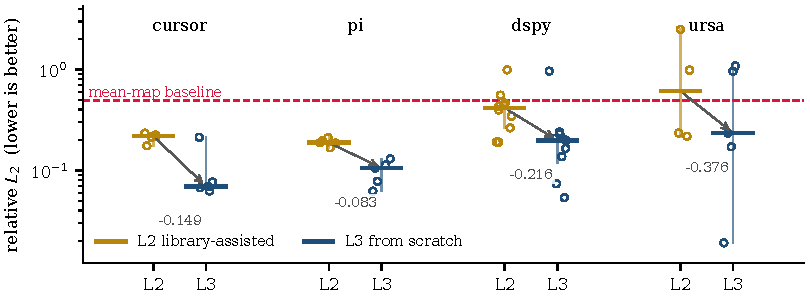
\includegraphics[width=0.68\textwidth]{figures/fig_levels}
\caption{Every scored run, by cell. Circles are replicates, the heavy bar the
cell median with its bootstrap interval, the arrow the within-harness
\Ltwo{}$\rightarrow$\Lthree{} contrast with its median difference. From-scratch
is better in all four substrates, and the two substrates with the widest spread
are the two producing runs worse than the mean-map baseline.}
\label{fig:levels}
\end{figure}

\paragraph{Does the harness matter, with the model held fixed?}
\label{sec:harness-effect}
Yes, and more than the access level does. With \emph{one model} across all eight
cells the per-cell medians span $0.0692$ to $0.6101$, a factor of $8.8$, against
the $1.7\times$ pooled level effect, ordering harnesses \hn{cursor}, \hn{pi},
\hn{dspy}, \hn{ursa} at \Lthree{} and the same but for a \hn{pi}/\hn{cursor}
swap at \Ltwo{}. The spread is not only in the median: \hn{cursor} and \hn{pi}
produced 20 scored runs with \emph{zero} physically invalid artifacts and a
worst case of $0.234$, while \hn{dspy} and \hn{ursa} account for all 15 invalid
artifacts and every run worse than the mean-map baseline. This is the comparison
usually confounded, and the empirical version of a claim recently argued on
other grounds---that the harness, not the model it wraps, is often the binding
constraint \citep{zhang2026harness}.

\paragraph{Against the non-agentic baseline.}
\label{sec:vs-baseline}
The pre-written pipeline, run at \Lzero{} with seeded heuristic decisions and
\emph{no LLM calls at all}, scores mean relative $L_2$ $0.1774$, $0.1865$ and
$0.1863$ on three seeds at a budget matched to the agents' 450 successful
solves---about 63\% accuracy, in 83--101 seconds, for \$0.00 of model spend; given
five times the data it reaches $0.1666$, so the budget is not what limits it.
Against that line, \textbf{two of eight agent cells beat the zero-LLM baseline}
(\Lthree{}-\hn{cursor}, \Lthree{}-\hn{pi}), one matches it and five are worse;
both that beat it are from-scratch. This constrains the reading of
Section~\ref{sec:l2l3}: the library is \emph{not} simply bad code dragging
\Ltwo{} down, since it outperforms five of the eight agent cells on the same
frozen set. The gap is better explained by what library access does to the
agent's search over methods.

\paragraph{Cost and budget compliance.}
\label{sec:cost}
Cost is dominated by one substrate---\hn{ursa} spent \$128.51 across 14 runs,
65\% of the campaign, against \$44.82 (\hn{dspy}), \$14.36 (\hn{cursor}) and
\$10.10 (\hn{pi})---and it buys nothing legible (Appendix~\ref{app:costfig}):
the two cheapest substrates occupy the two best positions and the most expensive
cell sits below \Lthree{}-\hn{pi} at one-thirteenth the price. Costs are measured where a substrate reports dollars and otherwise derived from
token counts at a committed price table; the \hn{cursor} figure is an estimate
at provider rates, not that vendor's billing. On the 450-solve bound the median cell is
compliant once uncapped validation and test solves are allowed for
($239$--$689$ attempted); the exceptions are in \Ltwo{}-\hn{dspy}, whose worst
runs attempted $1914$ and $1650$---overruns of $+1464$ and $+1200$ against a
bound stated in the prompt.

\section{Verification: delivery, validity, and honesty}
\label{sec:verification}

The benchmark separates three questions the literature usually collapses into
one. Plotting two of them against each other (Figure~\ref{fig:verif},
Appendix~\ref{app:verif}) makes the point: every run in that plot passed every
contract gate, and the physically invalid ones are scattered across the whole
range of self-reported honesty.
\subsection{Passing the gates is not being right}
\label{sec:validity}
\vspace{-2pt}
\code{contract.passed} certifies \emph{delivery}, not that the artifact is
physically meaningful. We record structural diagnostics beside the contract,
never as gates---adding a gate would change \code{contract.passed} and silently
make every archived run incomparable. Validity is judged on \emph{magnitude}, as
the conjunction of four checks: \textbf{sanity}, relative $L_2 < 0.8$, a
surrogate at all against a baseline of $0.49$; \textbf{full-grid error}, the same
metric recomputed with the plasma's exterior in the numerator and the interior
norm still in the denominator, so a spurious field written where flux is
undefined is charged rather than masked away; \textbf{exterior inflation}, the
ratio of the two ($1.0$ clean, $1.2$ a NaN-convention slip, $17$ a fabricated
plasma); and \textbf{prediction spread}, at least a tenth of ground truth's,
since a constant predictor is finite, correctly shaped and ignores its input.
NaN-mask agreement is recorded but \textbf{demoted out of the rule}: pixel
counting cannot tell a convention slip from an invented plasma---both can land
at $0.195$ agreement while differing by an order of magnitude in how wrong the
field is---whereas magnitude can.

\paragraph{The campaign-wide rate.}
\textbf{15 of 49 scored runs (31\%) passed every contract gate while being
physically invalid.} The rate is strongly substrate-specific and almost
completely level-independent: \hn{cursor} $0/10$ and \hn{pi} $0/10$ against
\hn{dspy} $\mathbf{11/20}$ and \hn{ursa} $\mathbf{4/9}$, while by access level it
is $7/24$ at \Ltwo{} and $8/25$ at \Lthree{}. Two substrates produce none of it and two all of it, while the axis the
benchmark was built to vary makes no difference; an evaluation reporting only
\code{contract.passed} would have scored this campaign $49/49$ delivered.

The same failure recurs across campaigns: a predictor emitting zeros instead of
NaN outside the boundary once passed \textbf{9/9 gates} at relative $L_2$
\textbf{0.9596}, twice as bad as predicting the mean field; here one
\Lthree{}-\hn{dspy} replicate emitted \emph{no NaN at all} against ground truth
that is $80.5\%$ NaN, and an \Ltwo{}-\hn{ursa} replicate reached a prediction
spread $16.2\times$ ground truth's (Appendix~\ref{app:invalid}). All of it is
invisible to the contract and caught by three numbers computed from predictions
the benchmark already has.

\paragraph{The honesty gap.}
\label{sec:honesty}
Because the contract checks that self-reported metrics are \emph{present} but
never \emph{true}, the difference between an agent's reported error and its
independently scored error is directly measurable:
$\mathrm{gap} = \overline{\mathrm{relL2}}^{\,\text{self}} -
\overline{\mathrm{relL2}}^{\,\text{scored}}$, negative meaning the agent claimed
to be better than it was. Across the 48 scored runs reporting a comparable
number the median gap is $-0.0012$: \textbf{most agents report their own error
accurately}. The tail is what matters: ten runs exceed $|{\rm gap}| = 0.1$, the worst being a
\Ltwo{}-\hn{ursa} run reporting $0.0515$ against a scored $0.9857$---a claim of
roughly nineteenfold better accuracy than it achieved---and, in the other
direction, one reporting $4.2557$ against $2.4941$. A plausibility filter that
rejects self-reports outside $[0,5]$ admits both extremes, so it separates
nothing here.

\paragraph{The two pathologies are different runs.}
Of the 15 invalid artifacts only 4 have $|{\rm gap}| > 0.1$; of the 10 large-gap
runs only 4 are invalid. An agent can be wrong and honest about it, or
approximately right and still misreport: \emph{neither measurement substitutes
for the other}. Both cluster in the same two substrates, but on different
replicates.

\paragraph{Failure taxonomy, and a control arm.}
\label{sec:taxonomy}
None of the ten unscored runs is a model capability failure: five were killed
by the driver watchdog before writing a deliverable, three died on a single
transient connection error, one timed out, one produced nothing usable
(Appendix~\ref{app:taxonomy}). Among runs that
\emph{did} score, the substantive failures are the 15 invalid artifacts, and
they split by mechanism in a way a single scalar could not: \emph{masking}
failures, NaN convention wrong and exterior inflation $2$--$4\times$---the
\hn{dspy} pattern, whose modal masking rule is a training-derived validity mask
rather than the plasma boundary polygon---and \emph{scale} failures, mask
near-perfect but magnitude wrong, the \hn{ursa} pattern.

A blind, outcome-blind rubric review over three replicates per cell (7
dimensions, 1--5, median of three passes, 23 judgeable runs, \$2.53) ranks the
\Lthree{} substrates \hn{pi} $3.71$, \hn{cursor} $3.57$, \hn{dspy} $3.14$,
\hn{ursa} $2.71$---the frozen-score ordering up to the \hn{pi}/\hn{cursor}
swap---and rates \Lthree{} above \Ltwo{} ($3.07$ vs $2.86$). Where it
\emph{disagrees} is instructive: it judged the adaptive sampling ``genuine'' in
21 of 23 runs, while the code analysis of Section~\ref{sec:agentlogic} finds the
criterion actually reacting to what was measured in 2 of 37. A reviewer reading
code accepts nominal adaptivity that a parser does not. The reviewer is also the
model that produced every run it grades, so its scores only corroborate the
deterministic analysis (Section~\ref{sec:limitations}).

Finally, the benchmark asks agents to sample adaptively, so it should say
whether that is worth asking for. Forcing the pipeline's own meta-loop to use
residual-UCB acquisition against a blind space-filling append---four paired
replicates, identical solve budgets, no LLM calls---gives a clean negative:
aggregate accuracy improves by $+1.47$ points on average while
\textbf{worst-cell} accuracy, pre-registered as the headline because an adaptive
method should pay off where the surrogate is weakest, moves by $-0.23$ and wins
in $2/4$ (Appendix~\ref{app:controlarm}). The two summaries point in opposite
directions, exactly the failure mode the pre-registration was written to
expose.

\section{What the agents actually did}
\label{sec:agentlogic}

A frozen-set score cannot distinguish two runs that reach the same error by
different reasoning---one choosing its adaptive points by ensemble disagreement
and stopping because validation error crossed the threshold, another relabelling
uniform sampling as ``adaptive'' and stopping because it ran out of rounds. We
measure that difference with two extractors over each finished workspace, both
\textbf{LLM-free and execution-free}: they parse the agent's Python with the
\code{ast} module and match role-scoped patterns, so the whole archive
re-extracts identically and for nothing. Scope is load-bearing---a
whole-workspace grep for \code{subprocess} is true of nearly every run---so each
question is answered only from the code playing the relevant role,
non-production files are excluded, and every answer carries \code{file:line}
evidence. The vocabulary is anchored on the typed action space of the scripted
levels, so every level lands in the same table and anything unmatched stays
\code{unknown}.

\begin{table}[tbp]
\centering
\caption{What each cell chose, and whether the code agrees with the prose.
\emph{Agr.} is the share of a cell's replicates on its modal chain of methods
(method reproducibility, not score reproducibility); \emph{Switch.} counts
replicates whose acquisition criterion changed between rounds; \emph{M-inf.}
counts replicates whose point-choosing function calls the surrogate; the last
column is the modal verdict of comparing the criterion each run names against
the one its code computes.}
\label{tab:logic}
\footnotesize
\setlength{\tabcolsep}{4pt}
\begin{tabular}{@{}lllccccl@{}}
\toprule
\textbf{Cell} & \textbf{Model} & \textbf{Acquisition} &
\textbf{Stop} & \textbf{Agr.} & \textbf{Switch.} &
\textbf{M-inf.} & \textbf{Code vs prose} \\
\midrule
\Ltwo{}-\hn{cursor} & kernel ridge & \code{uncertainty\_gp} & no thresh. & 0.20 & 0/2 & --- & unverifiable 5/5 \\
\Ltwo{}-\hn{dspy}   & kernel ridge & \code{residual\_ucb}   & no thresh. & 0.10 & 1/9 & 10/10 & partial 8, agree 2 \\
\Ltwo{}-\hn{pi}     & kernel ridge & \code{residual\_ucb}   & no thresh. & 0.20 & 1/5 & --- & unverifiable 5/5 \\
\Ltwo{}-\hn{ursa}   & ridge / k.r. & \code{uncertainty}     & unexpl.    & 0.38 & 0/3 & 2/5 & partial 3, \textbf{mismatch 2} \\
\midrule
\Lthree{}-\hn{cursor} & MLP (Torch) & \code{uncertainty\_ensemble} & thresh. met & 0.20 & 0/5 & 5/5 & \textbf{agree 4}, partial 1 \\
\Lthree{}-\hn{dspy}   & MLP (Torch) & \code{uncertainty\_ensemble} & no thresh.  & 0.10 & 0/8 & 8/10 & partial 9, mismatch 1 \\
\Lthree{}-\hn{pi}     & MLP (Torch) & \code{uncertainty\_ensemble} & thresh. met & 0.20 & 0/3 & 5/5 & \textbf{agree 3}, partial 2 \\
\Lthree{}-\hn{ursa}   & MLP (Torch) & \code{uncertainty}           & unexpl.     & 0.17 & 0/2 & 4/5 & partial 4, mismatch 1 \\
\bottomrule
\end{tabular}
\end{table}

\paragraph{Method choice tracks the access level, not the substrate.}
Table~\ref{tab:logic} shows a split no outcome metric reveals. \textbf{Every
\Ltwo{} cell's primary model is kernel ridge} (17 of the 20 replicates with a
classifiable primary)---the model the library's own zoo also selects in all six
\Lzero{} runs---and \textbf{every \Lthree{} cell's is a hand-written PyTorch
MLP} (25 of 26). Acquisition splits the same way: \Ltwo{} agents gravitate to
residual-UCB and GP variance, the two strategies the \Ltwo{} prompt names as
available in the library, while \Lthree{} agents converge on ensemble
disagreement, which no prompt mentions. Four independent substrates, given a
library, reproduce its defaults; given nothing, all four rediscover a different
method family and two beat the library with it. That is the mechanism behind the
level effect, and why we read it as anchoring rather than as the library being
bad code.

\paragraph{Method reproducibility is poor, even where score reproducibility is good.}
Chain agreement never exceeds $0.38$ and is $0.10$ in both ten-replicate cells:
the same agent, prompt and model produces a different pipeline nearly every
time. \Lthree{}-\hn{cursor} is the sharpest case---five distinct chains in five
replicates, while its error stayed inside $[0.062, 0.212]$ and every artifact
was valid. A benchmark reporting only the score spread concludes the agent is
consistent; it is consistently \emph{good}, but it is not doing the same thing
twice.

\paragraph{Nominal adaptivity is one fixed rule executed $n$ times.}
The task mandates up to three adaptive rounds whose points are chosen from the
current model or data. The criterion actually changed between rounds in
\textbf{2 of the 37} runs where it could be classified; the rest ran one rule
three times. The crude failure---a stated criterion that is pure randomness---
occurs in no cell; the subtler one, non-reactive adaptivity, is near-universal,
which is consistent with the control arm finding little for a reactive
criterion to earn at this budget.

\paragraph{The code often does not match the prose, and a library hides it.}
Comparing the criterion each run \emph{states} against the one its code
\emph{computes} gives \code{partial} 27, \code{unverifiable\_from\_code} 14,
\code{agree} 9 and \code{mismatch} 4 of the 54 runs with a verdict; \code{agree}
is modal in only two cells, both \Lthree{}, and the four mismatches fall in the
two substrates that also produce every invalid artifact. Seven \Ltwo{} runs name
a method for which their code carries no evidence at all, against \textbf{zero
in any \Lthree{} cell}. Worse for an evaluator, \Ltwo{}-\hn{cursor} and
\Ltwo{}-\hn{pi} are \code{unverifiable\_from\_code} in all ten runs: selection
happens inside the library, so no workspace function chooses points---a
structural consequence of scaffolding, not evasion, but it means \textbf{the
more scaffolding an evaluation provides, the less of the agent's reasoning stays
inspectable}. Twelve further dimensions
(Appendix~\ref{app:logicdetail}) show where the rest of the solution agrees---
the test set stays out of every fitting function, the pilot and
storage-validation gates hold in 59/59 runs, no \Lthree{} run hand-built a
mesh---and the one mandatory constraint quietly violated: roughly half the
corpus satisfies the deliverable self-test by \emph{importing}
\code{predict.py} rather than re-running it in a fresh process.

\section{Limitations}
\label{sec:limitations}

The full list is in Appendix~\ref{app:limitations}; four constrain what may be
concluded. \textbf{The primary statistical test was changed after seeing the
data}---we pre-specified a sign test over four harness pairs, found it cannot
return $p < 0.125$ at any effect size, and moved to a stratified rank test; all
three agree in sign, so the direction does not depend on the choice, but the
$p$-value does. \textbf{\Lthree{} receives two
scaffolding instructions \Ltwo{} does not} (a meshing milestone and a warning
against hand-built meshes), arguably necessary because \Lthree{} agents must
write solver plumbing \Ltwo{} agents delegate, so the contrast bundles library
access with a prompt difference and is not a pure library effect.
\textbf{Replicate counts are unequal and partly failure-determined}, and
denominators count attempts, so \Ltwo{}-\hn{dspy} is $10/15$ where among
executed runs it is $10/10$---a defensible convention that moves the pooled
\Ltwo{} pass rate materially. And \textbf{one model, which the judge shares}:
model control buys internal validity with external, the harness effect may
itself be model-dependent, and the blind review of Section~\ref{sec:verification}
is performed by the same model that produced every run it grades, so
self-preference cannot be excluded and no correction is applied.

\section{Conclusion}
\label{sec:conclusion}

On this task, giving an agent a proven library made it worse: from-scratch
agents beat library-assisted ones in all four substrates, pooled median relative
$L_2$ $0.137$ against $0.229$, and the deterministic analysis says why---given a
library, four independent substrates reproduced its default model and its named
acquisition strategies; given nothing, all four converged on a different method
family and two beat the library's own score. Holding the model fixed, the
harness mattered more than the access level, and the pipeline with no language
model at all still beat five of the eight agent cells. The durable point is
independent of how those numbers land. A benchmark that checks only whether an
agent produced the required files will silently certify work that is physically
wrong and self-reported dishonestly: here 31\% of scored runs passed every gate
while being physically invalid, and the runs that misreported their own error
were largely \emph{not} the same runs. Separating \emph{did it deliver},
\emph{is it valid} and \emph{did it tell the truth} costs three diagnostics
computed from predictions the benchmark already holds; asking \emph{did it do
what it said} costs a parser.


% -------------------------------------------------------- acknowledgements -
\begin{ack}
The campaign ran on a single workstation with no external compute grant. We
thank the Open FUSION Toolkit developers, whose solver and worked examples are
the substrate this benchmark is built on, and the maintainers of the four agent
frameworks evaluated here, none of whom were involved in or consulted about this
evaluation.
\end{ack}

% ------------------------------------------------------------ references ---
\small
\bibliographystyle{plainnat}
\bibliography{references}
\normalsize

\appendix
\section{The benchmark loop}
\label{app:loop}

\begin{figure}[htbp]
\centering
\resizebox{0.70\textwidth}{!}{%
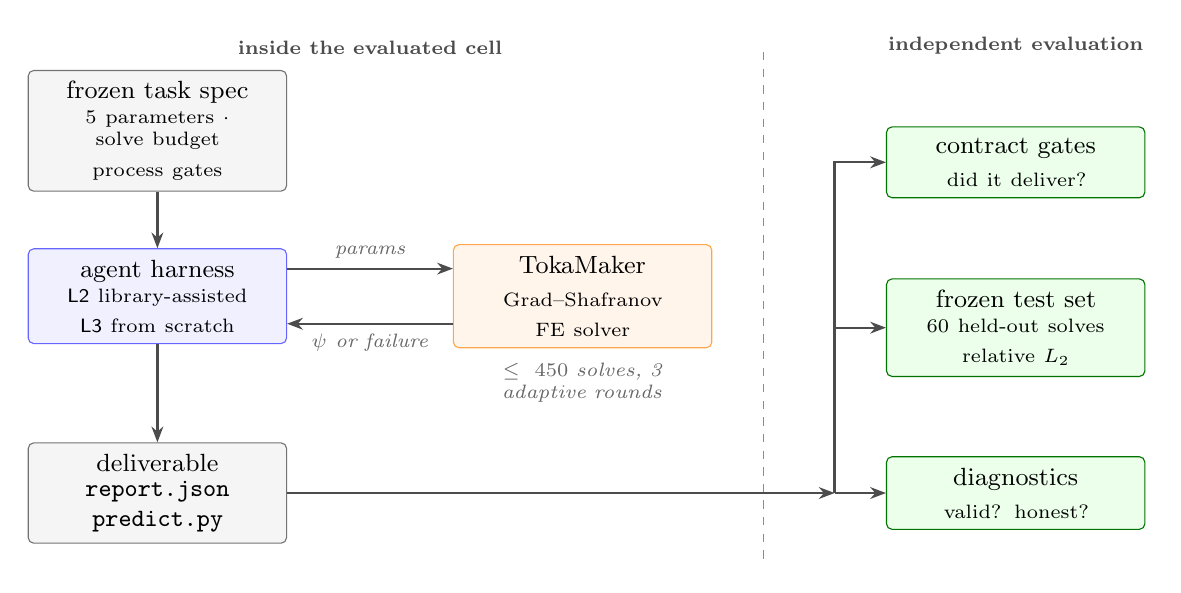
\begin{tikzpicture}[
  font=\small,
  box/.style={draw=black!55, rounded corners=2pt, align=center, inner sep=4pt,
              minimum height=9mm, text width=30mm},
  ag/.style={box, fill=blue!6,   draw=blue!60},
  sv/.style={box, fill=orange!8, draw=orange!70},
  ev/.style={box, fill=green!8,  draw=green!45!black},
  dl/.style={box, fill=black!4},
  fl/.style={-{Stealth[length=2mm]}, draw=black!70, thick},
  lb/.style={font=\scriptsize\itshape, text=black!60},
  hd/.style={font=\scriptsize\bfseries, text=black!70},
]

% ---- left: inside the evaluated cell ----
\node[dl] (task)  at (0,0)      {frozen task spec\\[1pt]{\scriptsize 5 parameters $\cdot$ solve budget\\ process gates}};
\node[ag] (agent) at (0,-2.1)   {agent harness\\[1pt]{\scriptsize \Ltwo{} library-assisted\\ \Lthree{} from scratch}};
\node[sv] (solv)  at (5.4,-2.1) {TokaMaker\\[1pt]{\scriptsize \GS{} FE solver}};
\node[dl] (deliv) at (0,-4.6)   {deliverable\\[1pt]{\scriptsize \code{report.json}\\ \code{predict.py}}};

\draw[fl] (task) -- (agent);
\draw[fl] ([yshift=3.5mm]agent.east) -- ([yshift=3.5mm]solv.west)
      node[midway,above,lb]{params};
\draw[fl] ([yshift=-3.5mm]solv.west) -- ([yshift=-3.5mm]agent.east)
      node[midway,below,lb]{$\psi$ or failure};
\draw[fl] (agent) -- (deliv);

\node[lb, text width=36mm, align=center] at (5.4,-3.2)
     {$\le 450$ solves, 3 adaptive rounds};

% ---- separator ----
\draw[dashed, black!45] (7.7,1.0) -- (7.7,-5.5);
\node[hd, anchor=south] at (2.7,0.85) {inside the evaluated cell};
\node[hd, anchor=south] at (10.9,0.85) {independent evaluation};

% ---- right: evaluation the agent never sees ----
\node[ev] (gates) at (10.9,-0.4) {contract gates\\[1pt]{\scriptsize did it deliver?}};
\node[ev] (score) at (10.9,-2.5) {frozen test set\\[1pt]{\scriptsize 60 held-out solves\\ relative $L_2$}};
\node[ev] (diag)  at (10.9,-4.6) {diagnostics\\[1pt]{\scriptsize valid? honest?}};

\coordinate (bus) at (8.6,-4.6);
\draw[fl] (deliv.east) -- (bus);
\draw[fl] (bus) -- (diag.west);
\draw[fl] (bus) |- (score.west);
\draw[fl] (bus) |- (gates.west);

\end{tikzpicture}%
}
\caption{The benchmark loop. The agent must \emph{buy} its own training data from
an expensive \GS{} solver under a fixed budget, choosing where to sample across
three adaptive rounds, and emits a deliverable that is checked, scored and
diagnosed entirely outside the cell on a test set it never sees. Every
condition passes through the identical right-hand column.}
\label{fig:loop}
\end{figure}


\section{Reproducibility}
\label{app:repro}

{\small
\begin{verbatim}
pip install -e ".[ml,dev,harnesses]"
python -m autotokamak.bench freeze-testset   # ground truth (committed)

tools/campaign_guard.py preflight --harnesses "ursa dspy pi cursor" \
                        --task benchmarks/tasks/L3_mini_v3.yaml
tools/run_campaign.sh --tag <tag> --reps 5 --parallel 6 --budget-usd 250 \
                      --harnesses "ursa dspy pi cursor"

python tools/cost_report.py        --tag <tag>
python tools/aggregate_matrix.py   --tag <tag>   # main table + all three tests
python tools/render_paper_figures.py --tag <tag> --out <paper>/figures
python tools/render_paper_tables.py  --tag <tag> --out <paper>/tables

python tools/run_library_baseline.py --n-samples 450 --seeds 0 1 2   # the L0 arm
python tools/run_control_arm.py      --reps 4                        # Section 7.4
python tools/judge_code.py score --tag <tag> --judge-provider openai \
                                 --samples 3 --per-cell 3            # Section 7.3
\end{verbatim}
}

Task texts are frozen and versioned; every run records the task's SHA-256, its
prompt version, its model string, and its replicate index. The frozen test set
carries provenance attributes (solver version, parameter and grid hashes,
scoring epoch) and is never regenerated. The statistics are seeded
(bootstrap and both permutation tests use seed \code{20260917}, 10\,000 and
20\,000 resamples respectively), so the analysis reproduces exactly from the
archived runs. Every figure and appendix table in this paper is generated from
those artifacts by the two scripts above rather than transcribed.

The one thing that does \emph{not} reproduce exactly is the agent runs
themselves: they are stochastic, and the substrates are versioned third-party
software that moves. That is why the campaign is replicated and reported with
intervals rather than as point estimates.

\section{Benchmark documentation}
\label{app:datasheet}

\paragraph{Access and hosting.}
The benchmark---task specifications, the deliverable contract, the frozen
evaluation assets, all harness adapters and every analysis script---is at
\url{https://github.com/hindyros/autotokamak}. The results in this paper are from
the campaign tagged \code{matrix-v4-20260919} at commit \code{dbc8289}. An
archival DOI is to be minted at camera-ready from the release tag.

\paragraph{Licensing.}
The benchmark code and task specifications are MIT licensed. The ground-truth
solver, Open FUSION Toolkit / TokaMaker \citep{hansen2024tokamaker}, is LGPL and
is used as an unmodified library dependency, which MIT-licensed code may do; we
redistribute no part of it. The frozen test set is derived data produced by that
solver from parameter vectors we generated, and is released under the same MIT
terms as the rest of the benchmark.

\paragraph{Maintenance.}
The contract, the evaluation grid and the frozen test set are versioned assets:
changing any of them makes archived scores incomparable, so the policy is that
they are not edited---a change means a new scoring epoch, recorded in the
archive's provenance attributes, and results are never pooled across epochs. New
diagnostics are added as recorded measurements, never as gates, for the same
reason. A new agent substrate is one adapter module implementing
\code{run(task, workspace, run\_dir, model, timeout)} plus one registry entry;
contributions are accepted on that interface.

\paragraph{Author statement.}
The authors bear all responsibility in case of violation of rights, and confirm
that the assets released with this paper are released under the license stated
above.

\paragraph{Compute.}
The entire campaign ran on a single workstation (Apple silicon, macOS): 59 agent
runs consuming 19.1 hours of wall clock with several cells concurrent, plus the
solver time inside each run, which is CPU-bound and is the dominant cost of a
cell in seconds if not in dollars. Model spend was \$197.78 in total. The two
supporting arms (Section~\ref{sec:vs-baseline} and
Appendix~\ref{app:controlarm}) make no model calls at all and cost \$0.00: the
budget-matched \Lzero{} arm takes 282\,s of wall clock for its three seeds
(1.8\,h for the unlimited-data variant) and the control arm 2.0\,h for its
eight runs. No GPUs or clusters were used, and reproducing the non-agentic
parts of this paper requires neither.

\paragraph{Ethical considerations and broader impact.}
The benchmark contains no human-subject or personally identifying data. Its
intended positive impact is on evaluation practice: we show that a benchmark
scoring only deliverable compliance certifies physically wrong artifacts at a
rate of roughly one in three, which is an argument for cheap independent
validity checks in any agent evaluation whose output is a scientific artifact.
The foreseeable negative is the ordinary one for capability benchmarks---that
scores become a target, and that a substrate could be tuned to this task's
contract rather than to the underlying problem; the frozen, never-regenerated
test set and the diagnostics that sit outside the contract are our partial
defence. The dual-use surface is that of the underlying solver, which is
publicly available open-source software \citep{hansen2024tokamaker}, and this
work adds nothing to it.

\paragraph{LLM usage.}
Large language models are the object of study: all eight agent cells are driven
by \code{gpt-5.2} (Section~\ref{sec:design}), and the blind code review in
Section~\ref{sec:taxonomy} uses the same model as a judge, with the
self-preference caveat recorded in Section~\ref{sec:limitations}. The
deterministic analyses of Sections~\ref{sec:validity} and \ref{sec:agentlogic}
use no language model at any point.

\section{Enforcing an equal compute budget}
\label{app:budget}

The long form of the summary in Section~\ref{sec:design}, reported because the
failure modes generalise to anyone building an agent evaluation.

Fair comparison requires every substrate to get the same budget, and this was
the single hardest engineering requirement in the benchmark. Two adapters
originally accepted a \code{timeout\_seconds} argument and silently ignored it.
Fixing that exposed two deeper failures, both found only by running a full
campaign: a timeout raised as an ordinary exception is \emph{swallowed}, because
agent frameworks wrap their step loops in broad \code{except Exception} handlers
and \code{signal.alarm} is one-shot, so a single absorbed alarm disables the cap
permanently---one harness ran over ten hours against a 90-minute budget; and
killing the agent process does not stop the work, because
\code{subprocess.run(capture\_output=True, timeout=...)} waits again on pipes
that the solver's grandchildren still hold open, so the timeout path itself
blocks---one cell sat in that deadlock for 9 hours 19 minutes. The fixes are to
raise a \code{BaseException} subclass, for the same reason \code{KeyboardInterrupt}
is one, and to run each agent in its own process group and signal the group.

The general lesson generalises past this benchmark: \textbf{an agent harness is
third-party code and cannot be trusted to honour a deadline from inside}. Our
final design enforces the budget at three independent levels---in-adapter
(graceful, and still records cost and partial output), process-group kill, and a
driver-side watchdog that nothing inside the cell can intercept. Benchmarks that
enforce time limits only in-process silently grant unequal compute to whichever
substrate is least well behaved, which is precisely backwards. We also equalised
\code{feedback\_rounds} to 1 for this campaign: only two of the four adapters
implement outer review-and-fix rounds at all, so any higher value handed those
two a second pass the others never got---the mechanical cause of their longer
runtimes and larger spend in earlier campaigns. One is the only value every
adapter honours identically.

\section{Task characterisation in full}
\label{app:characterisation}

From a direct sweep independent of any agent: pool $n = 9993$, test $n = 1499$.
Error is reported as a ratio to the mean-predictor baseline, so $1.0$ is ``no
better than predicting the average field''. Summarised in
Section~\ref{sec:characterisation}.

\begin{table}[htbp]
\centering
\caption{Scaling of surrogate error with training-set size. ``Best ratio'' is
relative $L_2$ divided by the mean-predictor baseline, minimised over the model
zoo.}
\label{tab:scale}
\small
\setlength{\tabcolsep}{5pt}
\begin{tabular}{@{}lrrrrrrrr@{}}
\toprule
$N$ & 50 & 100 & 200 & 400 & 800 & 1600 & 3200 & 6400 \\
\midrule
best ratio & 0.575 & 0.526 & 0.485 & 0.465 & 0.369 & 0.303 & 0.278 & 0.268 \\
$R^2$      & 0.804 & 0.840 & 0.865 & 0.876 & 0.922 & 0.948 & 0.956 & 0.959 \\
\bottomrule
\end{tabular}
\end{table}

\begin{table}[htbp]
\centering
\caption{Error ratio by sampling design at matched budget.}
\label{tab:design}
\small
\begin{tabular}{@{}lrrr@{}}
\toprule
$N$ & space-filling & random & clustered \\
\midrule
100  & \textbf{0.550} & 0.699 & 0.963 \\
400  & \textbf{0.358} & 0.438 & 0.873 \\
1600 & \textbf{0.289} & 0.309 & 0.808 \\
\bottomrule
\end{tabular}
\end{table}

\begin{table}[htbp]
\centering
\caption{Out-of-distribution generalisation. Rows in bold are the transfer
directions; both collapse to the mean predictor or worse.}
\label{tab:ood}
\small
\begin{tabular}{@{}lrr@{}}
\toprule
train $\rightarrow$ test & ratio & $R^2$ \\
\midrule
low $\rightarrow$ low   & 0.376 & 0.927 \\
high $\rightarrow$ high & 0.401 & 0.919 \\
\textbf{low $\rightarrow$ high}  & \textbf{0.943} & \textbf{0.280} \\
\textbf{high $\rightarrow$ low}  & \textbf{0.937} & \textbf{$-0.097$} \\
\bottomrule
\end{tabular}
\end{table}

\section{Limitations in full}
\label{app:limitations}

\begin{itemize}
\item \textbf{The primary statistical test was changed after seeing the data.}
  We pre-specified a sign test over four harness pairs, found it cannot return
  $p < 0.125$ at any effect size, and moved to a stratified rank test. All three
  tests agree in sign, so the direction does not depend on the choice; the
  $p$-value does. All three are reported wherever the contrast appears.
\item \textbf{\Lthree{} receives two scaffolding instructions \Ltwo{} does not}
  (a meshing milestone and a warning against hand-built meshes), arguably
  necessary because \Lthree{} agents must write solver plumbing \Ltwo{} agents
  delegate. The contrast bundles library access with a prompt difference and is
  not a pure library effect.
\item \textbf{Unequal, partly failure-determined replicate counts.} Two
  substrates have $n=10$ and two $n=5$. Denominators count attempts, so
  \Ltwo{}-\hn{dspy} is $10/15$ where among executed runs it is $10/10$; both
  conventions are defensible and the choice moves the pooled \Ltwo{} pass rate
  materially, so we state ours wherever a pass rate appears.
\item \textbf{One model, and the judge shares it.} Model control buys internal
  validity with external: the harness effect may itself be model-dependent. The
  blind review of Section~\ref{sec:taxonomy} is moreover performed by the same
  model that produced every run it grades, so self-preference cannot be excluded
  and no correction is applied---its scores corroborate the deterministic
  analysis and are never a measurement in their own right.
\item \textbf{Accounting caveats.} Wall-clock time is contaminated by
  concurrency on one CPU-bound machine and no executed-time measure is recorded,
  so cost and turn counts are the efficiency axes we report; one
  \Lthree{}-\hn{ursa} run was killed at a cap later runs did not face; and two
  substrates reuse a run identifier across sibling directories, so a join on it
  reuses one replicate's cost (we report the directory-keyed \$197.78 and note
  the \$199.76 discrepancy). Only two of the four ladder rungs are filled at
  this prompt version.
\item The benchmark is \textbf{fixed-boundary, single profile family, five
  parameters}: a real physics problem, but not a full one.
\end{itemize}

\section{Failure taxonomy in full}
\label{app:taxonomy}

None of the ten unscored runs is a model capability failure: five
\Ltwo{}-\hn{dspy} runs were terminated by the driver watchdog before writing a
deliverable (reconciled as explicit non-passing stubs rather than dropped, which
is why that cell's denominator is 15); three \Ltwo{}-\hn{ursa} runs died after
one turn on a single transient connection error, \$0.05 each, because that
adapter has no retry surviving it; one \Lthree{}-\hn{ursa} run timed out; and one
completed with 150 solves attempted, one succeeded, and no usable deliverable.
Among runs that \emph{did} score, the substantive failures are the 15 invalid
artifacts, and they split by mechanism in a way a single scalar could not
separate: \emph{masking} failures, NaN convention wrong and exterior inflation
$2$--$4\times$---the \hn{dspy} pattern, whose modal masking rule is a
training-derived validity mask rather than the plasma boundary polygon---and
\emph{scale} failures, mask near-perfect but magnitude wrong, the \hn{ursa}
pattern. Section~\ref{sec:agentlogic} traces both to choices in the code.

\paragraph{The blind code review.}
Full per-cell rubric scores are in
\code{experiments/<tag>/judge\_scores.csv}; the judge model, its blindness
conditions and the self-preference caveat are stated in
Section~\ref{sec:taxonomy} and Section~\ref{sec:limitations}. The one run of the
24 sampled that could not be judged is the errored \Ltwo{}-\hn{ursa} replicate,
whose workspace is empty.

\section{Forced-action control arm: did adaptive sampling help?}
\label{app:controlarm}

The benchmark asks agents to sample adaptively, so it should say whether adaptive
sampling is worth asking for. We ran the pipeline's own meta-loop twice over with
the action \emph{forced}, so the arms differ only in how new solver calls are
chosen: treatment forces residual-UCB acquisition, control a blind space-filling
append. Four paired replicates, identical per-iteration solve budgets, an
envelope evaluation set, no LLM calls in either arm. The pre-registered headline
is \textbf{worst-cell} accuracy, not aggregate accuracy, because an adaptive
method should pay off precisely where the surrogate is weakest and the aggregate
can hide that.

It is a clean negative. Aggregate accuracy improves by $+1.47$ percentage points
on average (3/4 replicates positive), but worst-cell accuracy---the quantity we
said in advance we would judge it on---moves by $-0.23$ points and wins in only
$2/4$. The two summaries point in opposite directions, which is exactly the
failure mode the pre-registration was written to expose. At this budget, on this
task, forced adaptive acquisition does not reliably beat blind space-filling
where it matters most.

\section{How the agents wrote it: prose, auditability and solution shape}
\label{app:logicdetail}

\paragraph{Stated criterion versus implemented criterion.}
Comparing the criterion each run \emph{states} against the one its code
\emph{computes}, at the level of the criterion family, gives \code{partial} 27,
\code{unverifiable\_from\_code} 14, \code{agree} 9 and \code{mismatch} 4 of the
54 runs with a verdict; \code{agree} is modal in only two cells, both \Lthree{}.
The four outright mismatches---stated and implemented criteria with nothing in
common---fall in the two substrates that also produce every invalid artifact.
Separately, three \Ltwo{}-\hn{dspy}, two \Ltwo{}-\hn{pi} and two \Ltwo{}-\hn{ursa}
runs name a method in their README or report for which the code carries no
evidence at all, against \textbf{zero such claims in any \Lthree{} cell}.

\paragraph{Library access removes auditability.}
\Ltwo{}-\hn{cursor} and \Ltwo{}-\hn{pi} are \code{unverifiable\_from\_code} in all
ten runs, and whether their selection is model-informed is simply unknown:
selection happens inside the library, so no workspace function chooses points.
This is a structural consequence of giving an agent a library, not evasion---but
it means the more scaffolding an evaluation provides, the less of the agent's
reasoning stays inspectable. Where a chooser can be classified at all, it usually does call the surrogate:
22 of the 25 such runs at \Lthree{} and 12 of 15 at \Ltwo{}. Relatedly, \hn{ursa} rounds largely did not record validation
error against baseline at the moment of choosing (median evidence-grounding
$0.33$ at \Ltwo{} and $0.17$ at \Lthree{}, against $1.0$ elsewhere), so its
stopping decisions cannot be falsified from its own artifacts at all.

\paragraph{The whole solution shape.}
Twelve further dimensions ask how each run solved the rest of the task
(Appendix~\ref{app:shape}). Three are identical across all eight cells at the level of the
\emph{modal} value---the test set stays out of every model-fitting function,
the pilot gate is enforced, and a solve is counted only after its stored
artifact is re-read and confirmed finite. A modal value hides the minority,
though, and the per-run counts do not: of the 51 runs whose workspace can be
read, 50 enforce the pilot gate, 46 validate storage (three claim it without
evidence, two are unreadable), and 42 of the 43 with a readable answer keep the
test set out of the fitting functions---\emph{one references it inside one}.
The anti-Delaunay prohibition, by contrast, held outright: 26 of 26 \Lthree{}
runs meshed through the solver's own API. The interesting failure is the \emph{deliverable self-test}: the task
requires re-running the documented \code{predict.py} command in a fresh process
before declaring done, and roughly half the corpus satisfies it by
\emph{importing} the module instead. Code that has not been re-run the way it is
documented to be run is the precondition for most of the interface failures this
benchmark has ever recorded---a mandatory constraint being partially violated in
plain sight, measurable only because the question is asked of the code that plays
that role.

\section{The scoring rule}
\label{app:scoring}

Predictions are scored against a frozen test set of 60 parameter vectors
(generated with seed \code{20260809} and committed; all 60 solves converged)
solved once and stamped with provenance: solver version, the SHA-256 of both the
parameter file and the grid, and a scoring epoch, so that a score is only ever
pooled with scores computed the same way. The archive is never regenerated. The
metric is per-sample relative $L_2$ over the finite ground-truth points:
\begin{equation}
  \mathrm{err}_i \;=\;
  \frac{\bigl\lVert \hat{\psi}_i - \psi_i \bigr\rVert_2}
       {\bigl\lVert \psi_i \bigr\rVert_2},
  \qquad
  \text{masked to } \{(\Rgrid,\Zgrid) : \psi_i(\Rgrid,\Zgrid) \text{ finite}\}.
  \label{eq:rell2}
\end{equation}
\textbf{A NaN prediction at a finite ground-truth point is scored as a
full-magnitude miss} (the prediction is treated as zero), never skipped---%
otherwise an all-NaN prediction scores as perfect. Accuracy is quoted against
the trivial mean-flux-map predictor on the same set,
$100 \times (1 - \mathrm{relL2} / \mathrm{baseline})$, where the baseline
scores $0.4933$.

\section{Invalid artifacts that passed every gate}
\label{app:invalid}

From a prior campaign: an agent passed \textbf{9/9 gates} at relative $L_2$
\textbf{0.9596}---accuracy $\mathbf{-94.5\%}$, twice as bad as predicting the
mean field---because its predictor emitted zeros instead of NaN outside the
boundary, at a spread ratio of $0.027$. The same family recurs here: one
\Lthree{}-\hn{dspy} replicate emitted \emph{no NaN at all} against ground truth
that is $80.5\%$ NaN, and an \Ltwo{}-\hn{ursa} replicate reached a prediction
spread $16.2\times$ ground truth's. All of it is invisible to the contract, and
all of it is caught by three numbers computed from predictions the benchmark
already has.

\section{The verification plane}
\label{app:verif}

\begin{figure}[htbp]
\centering
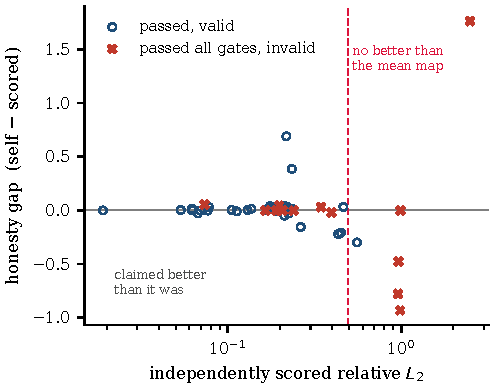
\includegraphics[width=0.52\textwidth]{figures/fig_verification}
\caption{The verification plane. Every point passed every contract gate.
Crosses are physically invalid artifacts; the dashed line is the mean-map
baseline. Large honesty gaps and invalid artifacts are largely different runs.}
\label{fig:verif}
\end{figure}

\section{Cost against accuracy}
\label{app:costfig}

\begin{figure}[htbp]
\centering
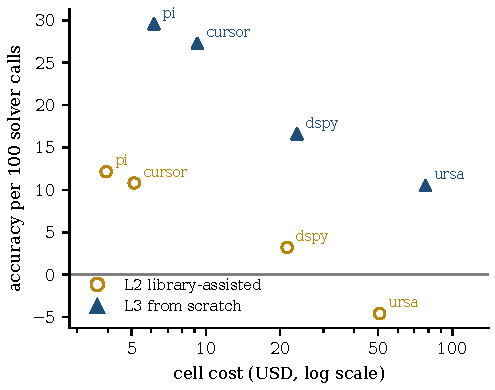
\includegraphics[width=0.52\textwidth]{figures/fig_cost}
\caption{What each cell's accuracy cost, at one model. A $13\times$ spread in
dollars buys no consistent advantage, and the most expensive substrate is the
least accurate at both access levels.}
\end{figure}

\section{The deliverable contract in full}
\label{app:gates}

\begin{table}[t]
\centering
\caption{The deliverable contract. \code{contract.passed} is the flat
\textsc{and} of all gates: no weighting, no partial credit. The scoring
subprocess is stripped of provider credentials, so \code{predict.py} must work
offline, and runs in its own process group so a timeout reaps the solver
children too.}
\label{tab:gates}
\small
\begin{tabular}{@{}ll@{}}
\toprule
\textbf{Gate} & \textbf{What it checks} \\
\midrule
\code{artifact:report.json} & present and non-empty \\
\code{artifact:predict.py}  & present and non-empty \\
\code{artifact:README.md}   & present and non-empty \\
\code{report\_parses}       & \code{report.json} is valid JSON \\
\code{report\_keys}         & \code{n\_solves\_\{attempted,succeeded\}} and \\
                            & \code{metrics.\{test,baseline\}\_rel\_l2.\{mean,median,p90\}} present \\
\code{no\_autotokamak\_import} & \Lthree{} only --- no workspace \code{.py} imports the platform \\
                            & library, by regex over plain imports, \code{importlib}, \code{\_\_import\_\_} \\
\code{predict\_runs}        & \code{python predict.py -{}-input params.json -{}-output pred.npz} exits 0 \\
\code{predict\_shape}       & returned \code{psi} is $(N, 96, 64)$ \\
\code{predict\_grid}        & returned \code{R}, \code{Z} match the frozen axes to $10^{-9}$ \\
\bottomrule
\end{tabular}
\end{table}

\section{Frozen assets}
\label{app:assets}

\begin{itemize}
\item \code{benchmarks/assets/eval\_grid.json} --- the frozen evaluation grid:
  64 points in $\Rgrid \in [0.15, 0.80]$\,m and 96 in $\Zgrid \in [-0.40,
  0.40]$\,m, both \code{linspace}. Flux arrays are stored $(N, 96, 64)$, that
  is $(N, n_Z, n_R)$.
\item \code{benchmarks/assets/test\_params.json} --- the 60 held-out parameter
  vectors, generated with seed \code{20260809}. SHA-256
  \code{d10a3651...d17b480}.
\item \code{benchmarks/assets/test\_set.h5} --- ground-truth flux fields, all 60
  solves converged; $80.46\%$ of grid points are NaN, outside the plasma.
  Provenance attributes record the stamp time, the solver version (26.6), the
  SHA-256 of both the parameter file and the grid, the sweep configuration and
  its hash, and the scoring epoch (\code{2026-08-18}). Never regenerated; every
  archived score is relative to it.
\item \code{benchmarks/assets/prices.json} --- the dated price table behind
  every derived cost figure, so a published dollar amount is traceable to the
  rates it was computed with.
\item \code{benchmarks/tasks/*.yaml} --- the task specifications.
\end{itemize}

\section{The task text, and the \texorpdfstring{\Ltwo{}/\Lthree{}}{L2/L3} difference}
\label{app:tasktext}

The \Lthree{} problem statement is reproduced verbatim below. The \Ltwo{} text
is byte-identical to it except for the ten hunks that follow, every one of which
concerns access level: the title, the description of the solver, the three
pipeline steps where the library would be used, the workspace and environment
bullets, the single-\code{OFT\_env} advice, and the constraints block. The
parameter ranges, the budget, the stopping criterion, the evaluation interface,
all five deliverables, the ``do not fabricate metrics'' paragraph and the three
process gates are identical.

\subsection{\Lthree{} problem statement (verbatim)}
% generated by tools/render_paper_tables.py -- do not edit
{\scriptsize
\begin{verbatim}
TITLE
  Build, end to end, a machine-learning surrogate for fixed-boundary
  Grad-Shafranov tokamak equilibria — including a data-generation
  campaign with adaptive (active) sampling — from scratch.

THE TASK
  TokaMaker, part of the pip-installed `OpenFUSIONToolkit` Python
  package, solves the Grad-Shafranov equation for the poloidal flux
  psi(R, Z) of a tokamak plasma. You will use it as your ground-truth
  physics solver.

  Consider fixed-boundary equilibria of D-shaped plasmas described by
  5 input parameters, with TokaMaker's default pressure/current
  profile shapes:

    r0    : major radius        [m]   in [0.35, 0.55]
    a     : minor radius        [m]   in [0.10, 0.20]
    kappa : elongation          [-]   in [1.0, 1.6]
    delta : triangularity       [-]   in [0.0, 0.4]
    Ip    : plasma current      [A]   in [80e3, 200e3]
    (plasma centered at z0 = 0)

  Your job, in full:
    1. Learn how to drive TokaMaker for fixed-boundary solves (mesh a
       D-shaped last-closed-flux-surface, solve, extract psi). Choose
       your own numerical resolution; a single solve should take
       seconds, not minutes.
    2. Design and run a DATA-GENERATION CAMPAIGN structured as an
       initial space-filling design of AT MOST 150 solves followed by UP TO 3 ADAPTIVE
       (ACTIVE-SAMPLING) ROUNDS of EXACTLY 100 new solver runs each
       (failed/unconverged solves count against a round's 100).
       A one-shot space-filling or random design alone is NOT
       sufficient: each round's 100 new solver evaluations must be
       chosen ADAPTIVELY, informed by the current model or data (your
       strategy — e.g. uncertainty, model error, disagreement,
       anything you can justify). STOPPING CRITERION: keep a held-out
       VALIDATION set (separate from the final test set of step 4,
       which must never influence the campaign); after each round,
       retrain your surrogate and stop the campaign early once its
       validation error is reduced by at least 70% relative to the
       mean-predictor baseline (a model that always predicts the
       training-set mean psi map), i.e. val_error <= 0.30 *
       baseline_error. Otherwise continue to the 3-round cap. Log
       every acquisition decision (which point, when, why) and each
       round's validation error vs baseline to an acquisition log
       file.
    3. Train an ML surrogate mapping the 5 parameters to the PHYSICAL
       poloidal flux psi(R, Z) in Webers (not a normalized flux).
       Model family, input/output representation, and training
       procedure are entirely your choice.
    4. Evaluate honestly on a held-out test set of AT LEAST 20 solver
       runs at uniformly random parameters (fixed recorded seed),
       generated independently and never used for training, model
       selection, or acquisition.
    5. Report results and analyze whether your adaptive sampling
       actually helped (e.g. versus the model trained on the initial
       design only, or any comparison you can defend).

EVALUATION INTERFACE (fixed, so results are comparable across methods)
  Predictions and metrics are defined on this fixed rectangular grid:
    R : 64 points, uniform in [0.15, 0.80] m
    Z : 96 points, uniform in [-0.40, 0.40] m
  psi arrays are shaped (96, 64) = (nZ, nR). Grid points outside the
  plasma boundary carry NaN; all metrics are computed only where the
  ground truth is finite.

  Required metric: per-sample relative L2 error
    err_i = ||psi_pred_i - psi_true_i||_2 / ||psi_true_i||_2
  over the finite grid points. Report mean, median, and 90th
  percentile over the test set, and the same numbers for a trivial
  baseline (predict the training-set mean psi) so the surrogate's
  value is evident.

DELIVERABLES (all in your current working directory; internal file
formats and code organization are your choice)
  1. Your pipeline code, runnable end to end by one documented entry
     command.
  2. The dataset(s) you generated, plus the acquisition log.
  3. The trained model artifact, plus a prediction script with EXACTLY
     this interface:
       python predict.py --input params.json --output pred.npz
     where params.json is a JSON list of objects with keys
     r0, a, kappa, delta, Ip, and pred.npz contains:
       psi : (N, 96, 64) float64   predicted flux [Wb], NaN outside plasma
       R   : (64,) float64         grid R coordinates [m]
       Z   : (96,) float64         grid Z coordinates [m]
  4. report.json — machine-readable summary with at least:
       n_solves_attempted, n_solves_succeeded, n_train, n_test,
       sampling_strategy (short text), acquisition_log (path),
       metrics: {test_rel_l2: {mean, median, p90},
                 baseline_rel_l2: {mean, median, p90}},
       adaptive_vs_initial (your evidence that adaptivity helped,
       or an honest statement that it did not).
  5. README.md — your design, why you chose it, how to run, results.

  You MUST actually run the full campaign and training within this
  session and verify every deliverable exists before declaring done.
  Report failures honestly in report.json/README; do not fabricate
  metrics.

ENVIRONMENT FACTS
  * Your current working directory IS your workspace. Create all files
    here. Do not read, copy, or import code from the surrounding
    repository. In particular the Python environment contains an
    installed package called `autotokamak` that solves a related
    problem — importing it, reading its source, or reusing its
    artifacts is FORBIDDEN: this is a from-scratch capability test,
    and only `OpenFUSIONToolkit` may be used for physics.
  * `python` resolves to a Python 3.11 venv that already has:
    numpy, scipy, h5py, matplotlib, pyyaml, scikit-learn, torch,
    optuna, OpenFUSIONToolkit. Nothing may be installed.
  * A read-only `./OpenFUSIONToolkit/` symlink to the full OFT
    source tree is present in your workspace. BEFORE writing any
    solver or meshing code, study the worked TokaMaker examples
    under `OpenFUSIONToolkit/src/examples/TokaMaker/` (the
    `fixed_boundary/` example is directly relevant) and follow the
    workflow they demonstrate rather than inventing your own
    solver-facing plumbing.
  * TokaMaker limitation: only ONE `OFT_env` may ever be created per
    Python process. Structure your code so the environment object is
    created once and reused across all solves in a process, or run
    solves in child processes.

CONSTRAINTS
  * MESHING MILESTONE (mandatory, before any campaign code): locate
    the fixed-boundary example under
    `OpenFUSIONToolkit/src/examples/TokaMaker/`, reproduce its
    mesh-and-solve workflow as a standalone script in your workspace,
    run it, and verify it produces finite psi values. Only then
    generalize it to your parameterized D-shape. Do not design your
    own meshing approach when the examples demonstrate one.
  * Do NOT construct the computational mesh yourself (e.g. via scipy
    Delaunay) and pass raw triangles to the solver — TokaMaker
    validates mesh topology and will reject hand-built
    triangulations. Use the meshing route the OFT examples use.
  * PILOT GATE (mandatory): before the campaign, run a pilot of at
    least 20 solves at random parameters. If the success rate is
    below 50%, STOP, diagnose the per-failure error messages, fix,
    and re-run the pilot. Never start the 100-solve rounds while the
    pilot is failing.
  * STORAGE VALIDATION GATE (mandatory): a solver run may be counted
    as successful ONLY after its stored artifact has been re-loaded
    from disk and verified: the saved psi grid must contain a nonzero
    fraction of finite values. Apply this check to every batch you
    write. A stored all-NaN psi grid is a FAILED solve regardless of
    solver exit status, and your reported success counts must be based
    on validated stored artifacts, not solver return codes.
  * DELIVERABLE SELF-TEST (mandatory, before declaring done): in a
    fresh Python process, run the exact documented command for each
    deliverable — including `python predict.py --input <sample params>
    --output <out>` — and verify the output loads with the required
    shapes and finite values. If any deliverable fails its own
    interface test, fix it and re-test. Code you have not re-run after
    your last edit does not count as verified.
  * Do not run `pip install` or modify the environment.
  * Do not call `git`.
  * Do not prompt for user input; the task is fully autonomous.
  * If errors arise, debug, fix your code, and re-run. Stay within
    the campaign structure above (at most 3 adaptive rounds x 100
    solves, plus the initial design and validation/test sets) across
    ALL attempts that reach the solver.
\end{verbatim}
}


\subsection{Diff from the \Ltwo{} statement}
% generated by tools/render_paper_tables.py -- do not edit
% 10 hunks
{\scriptsize
\begin{verbatim}
--- L2_mini_v3
+++ L3_mini_v3
@@ -4,2 +4 @@
-  campaign with adaptive (active) sampling — using the installed
-  `autotokamak` platform library wherever it helps.
+  campaign with adaptive (active) sampling — from scratch.
@@ -10,2 +9,2 @@
-  psi(R, Z) of a tokamak plasma. It is your ground-truth physics
-  solver, and the installed `autotokamak` package already wraps it.
+  psi(R, Z) of a tokamak plasma. You will use it as your ground-truth
+  physics solver.
@@ -25,4 +24,3 @@
-    1. Drive the solver for fixed-boundary solves. You may use
-       `autotokamak.data.sweep.run_sweep` (config-driven sweeps; also
-       accepts an explicit (N, 5) sample matrix), or go through
-       `autotokamak.core` directly. A single solve should take
+    1. Learn how to drive TokaMaker for fixed-boundary solves (mesh a
+       D-shaped last-closed-flux-surface, solve, extract psi). Choose
+       your own numerical resolution; a single solve should take
@@ -36,13 +34,13 @@
-       chosen ADAPTIVELY, informed by the current model or data
-       (`autotokamak.data.acquire` implements residual-UCB and PCA-GP
-       variance acquisition you may reuse, or bring your own).
-       STOPPING CRITERION: keep a held-out VALIDATION set (separate
-       from the final test set of step 4, which must never influence
-       the campaign); after each round, retrain your surrogate and
-       stop the campaign early once its validation error is reduced
-       by at least 70% relative to the mean-predictor baseline (a
-       model that always predicts the training-set mean psi map),
-       i.e. val_error <= 0.30 * baseline_error. Otherwise continue to
-       the 3-round cap. Log every acquisition decision (which point,
-       when, why) and each round's validation error vs baseline to an
-       acquisition log file.
+       chosen ADAPTIVELY, informed by the current model or data (your
+       strategy — e.g. uncertainty, model error, disagreement,
+       anything you can justify). STOPPING CRITERION: keep a held-out
+       VALIDATION set (separate from the final test set of step 4,
+       which must never influence the campaign); after each round,
+       retrain your surrogate and stop the campaign early once its
+       validation error is reduced by at least 70% relative to the
+       mean-predictor baseline (a model that always predicts the
+       training-set mean psi map), i.e. val_error <= 0.30 *
+       baseline_error. Otherwise continue to the 3-round cap. Log
+       every acquisition decision (which point, when, why) and each
+       round's validation error vs baseline to an acquisition log
+       file.
@@ -51,4 +49,2 @@
-       `autotokamak.surrogate` provides dataset loading, PCA
-       reduction, a model zoo (GP, kernel ridge, polynomial ridge,
-       MLP), and Optuna search; model family and representation
-       remain entirely your choice.
+       Model family, input/output representation, and training
+       procedure are entirely your choice.
@@ -107 +103,6 @@
-    here.
+    here. Do not read, copy, or import code from the surrounding
+    repository. In particular the Python environment contains an
+    installed package called `autotokamak` that solves a related
+    problem — importing it, reading its source, or reusing its
+    artifacts is FORBIDDEN: this is a from-scratch capability test,
+    and only `OpenFUSIONToolkit` may be used for physics.
@@ -110,8 +111,8 @@
-    optuna, OpenFUSIONToolkit, and the `autotokamak` platform library
-    (importable; using it is ALLOWED and RECOMMENDED — that is the
-    point of this condition). Nothing may be installed.
-  * Useful autotokamak entry points: `autotokamak.data.sweep.run_sweep`
-    (sweep or explicit-matrix solves → HDF5),
-    `autotokamak.data.acquire` (acquisition strategies),
-    `autotokamak.surrogate.dataset/reduce/zoo/optuna_search/automl_loop`
-    (loading, PCA, model factories, search). Read their docstrings.
+    optuna, OpenFUSIONToolkit. Nothing may be installed.
+  * A read-only `./OpenFUSIONToolkit/` symlink to the full OFT
+    source tree is present in your workspace. BEFORE writing any
+    solver or meshing code, study the worked TokaMaker examples
+    under `OpenFUSIONToolkit/src/examples/TokaMaker/` (the
+    `fixed_boundary/` example is directly relevant) and follow the
+    workflow they demonstrate rather than inventing your own
+    solver-facing plumbing.
@@ -119,4 +120,3 @@
-    Python process. `autotokamak.core.solver.make_solver` handles
-    reuse via its `env=` argument; if you bypass autotokamak, create
-    the environment object once and reuse it, or run solves in child
-    processes.
+    Python process. Structure your code so the environment object is
+    created once and reused across all solves in a process, or run
+    solves in child processes.
@@ -124,0 +125,11 @@
+  * MESHING MILESTONE (mandatory, before any campaign code): locate
+    the fixed-boundary example under
+    `OpenFUSIONToolkit/src/examples/TokaMaker/`, reproduce its
+    mesh-and-solve workflow as a standalone script in your workspace,
+    run it, and verify it produces finite psi values. Only then
+    generalize it to your parameterized D-shape. Do not design your
+    own meshing approach when the examples demonstrate one.
+  * Do NOT construct the computational mesh yourself (e.g. via scipy
+    Delaunay) and pass raw triangles to the solver — TokaMaker
+    validates mesh topology and will reject hand-built
+    triangulations. Use the meshing route the OFT examples use.
@@ -147,2 +157,0 @@
-  * Do not modify the installed autotokamak/OpenFUSIONToolkit
-    packages; use them as libraries.
\end{verbatim}
}


\section{Solution-shape cross comparison}
\label{app:shape}

Twelve questions, each answered from the code that plays the relevant role, with
\code{file:line} evidence recorded per run. Cells are abbreviated by level and
harness: \code{2c} is \Ltwo{}-\hn{cursor}, \code{3u} is \Lthree{}-\hn{ursa}, and
so on. A dash means the dimension is not answerable for that cell, which at
\Ltwo{} generally means the library owns that part of the pipeline.

\begin{center}
\scriptsize
% generated by tools/render_paper_tables.py -- do not edit
\begin{tabular}{@{}ll>{\raggedright\arraybackslash}p{0.44\textwidth}@{}}
\toprule
\textbf{Dimension} & \textbf{Cells} & \textbf{Modal value} \\
\midrule
code\_shape & 2c, 2p & \code{single\_script} \\
 & 2d & \code{14\_modules} \\
 & 2u & \code{15\_modules} \\
 & 3c & \code{8\_modules} \\
 & 3d & \code{11\_modules} \\
 & 3p & \code{9\_modules} \\
 & 3u & \code{7\_modules} \\
\addlinespace[2pt]
entry\_point & 2c, 2p, 3p & \code{2\_runnable\_scripts} \\
 & 2d, 3u & \code{10\_runnable\_scripts} \\
 & 2u & \code{9\_runnable\_scripts} \\
 & 3c & \code{3\_runnable\_scripts} \\
 & 3d & \code{7\_runnable\_scripts} \\
\addlinespace[2pt]
grid\_mapping & 2c, 2d, 2p, 2u & --- \\
 & 3c, 3d, 3p, 3u & \code{solver\_field\_eval} \\
\addlinespace[2pt]
mask\_rule & 2c, 2p, 3c, 3d, 3p & \code{lcfs\_polygon} \\
 & 2d, 2u & \code{training\_valid\_mask} \\
 & 3u & \code{lcfs\_polygon+training\_valid\_mask} \\
\addlinespace[2pt]
mesh\_route & 2c, 2u, 3c, 3d, 3p, 3u & \code{oft\_gs\_domain} \\
 & 2d, 2p & --- \\
\addlinespace[2pt]
oft\_env\_strategy & 2c, 2d, 2p, 2u & --- \\
 & 3c, 3d, 3p, 3u & \code{singleton\_reused} \\
\addlinespace[2pt]
self\_test & 2c, 2d, 2u, 3p, 3u & \code{subprocess\_reruns\_predict} \\
 & 2p, 3c, 3d & \code{imported\_not\_subprocessed} \\
\addlinespace[2pt]
solve\_isolation & 2c, 2d, 2p, 2u, 3c, 3d, 3u & \code{in\_process\_serial} \\
 & 3p & \code{subprocess\_per\_batch} \\
\addlinespace[2pt]
storage & 2c, 2p, 3c, 3p & \code{npz\_per\_solve+pickle} \\
 & 3d, 3u & \code{npz\_per\_solve+pickle+index} \\
 & 2d & \code{npz\_per\_solve+hdf5} \\
 & 2u & \code{npz\_per\_solve+hdf5+index} \\
\addlinespace[2pt]
leakage\_guard & 2c, 2d, 2p, 2u, 3c, 3d, 3p, 3u & \code{test\_absent\_from\_fitting\_functions} \\
\addlinespace[2pt]
pilot\_gate & 2c, 2d, 2p, 2u, 3c, 3d, 3p, 3u & \code{enforced} \\
\addlinespace[2pt]
storage\_validation & 2c, 2d, 2p, 2u, 3c, 3d, 3p, 3u & \code{reload\_and\_check\_finite} \\
\addlinespace[2pt]
\bottomrule
\end{tabular}

\end{center}

\section{Glossary of canonical values}
\label{app:glossary}

Every code printed in Table~\ref{tab:logic} and Appendix~\ref{app:shape}. A code
a reader has to guess at is not a measurement.

% generated by tools/render_paper_tables.py -- do not edit
\begin{description}[leftmargin=1.2em,style=nextline,font=\ttfamily\small]
\item[N\_modules] The pipeline is spread over N source files, none of them dominant; contrast \code{single\_script}.
\item[N\_runnable\_scripts] N files are runnable as programs. More than one means the documented single command is really a sequence.
\item[adaptive\_in\_name\_only] Every stated criterion names nothing but randomness: the round was labelled adaptive and was not.
\item[agree] The criterion stated in the log/report is the one the code computes.
\item[chain\_agreement] Share of a cell's replicates that chose the modal chain of methods — method reproducibility, which is not the same as score reproducibility.
\item[criterion\_switched] The acquisition criterion CHANGED between rounds — logic reacting to what it measured, rather than one fixed rule executed n times.
\item[deep\_ensemble] Several independently initialised models, averaged.
\item[enforced] A pilot runs and its success rate is compared against a threshold before the campaign proceeds — the task's 50\% pilot gate.
\item[evidence\_grounded] The round's validation error against baseline was recorded, so its choice can be checked against what was known at the time. An ungrounded round's reasoning is unfalsifiable.
\item[feasibility] Candidate choice weighted by whether solves there are expected to converge, steering away from regions with failed solves.
\item[gradient\_sensitivity] Points where the response is steep or curving — a sensitivity or Jacobian-driven criterion.
\item[hdf5] One HDF5 file holding many samples. Scales best and carries attributes/provenance, at the price of concurrent-write care.
\item[imported\_not\_subprocessed] predict.py is referenced but only imported or described, never run as the documented command. Code that works in the session's process and fails in a clean one is exactly what this misses.
\item[in\_process\_serial] Solves run one after another inside the driving process. Simplest, and the slowest: no parallelism, and one bad solve can poison the shared solver state.
\item[index] An index/manifest (CSV or JSONL) sits beside the arrays, listing every sample and its status. What makes a campaign resumable and auditable rather than a directory to be re-scanned.
\item[kernel\_ridge] Kernel ridge regression — a GP's mean without its variance.
\item[lcfs\_polygon] A grid point is inside the plasma iff it lies within the LCFS polygon — point-in-polygon against the D-shape boundary, whatever the helper is called (contains\_points, \_points\_in\_poly, inside\_lcfs\_mask). Geometric, per sample, and independent of the surrogate's own output.
\item[lhs] Latin hypercube: stratified in every dimension at once.
\item[mc\_dropout] Dropout left active at inference and sampled repeatedly — an ensemble's spread at one model's training cost.
\item[mismatch] The stated criterion and the implemented one have nothing in common. The strongest available signal that a run's account of itself is wrong.
\item[mlp\_torch] A hand-written PyTorch MLP. The most common choice in this corpus, usually mapping 5 parameters to PCA coefficients.
\item[model\_informed] The function that chooses points actually calls the surrogate. A model-derived criterion that never does is not one, whatever it is named.
\item[npz\_per\_solve] One compressed .npz per solved sample.
\item[oft\_gs\_domain] Meshed through OFT's own API (gs\_Domain / define\_region / build\_mesh) as the worked examples do. What the task's meshing milestone asks for, and what TokaMaker's topology checks accept.
\item[partial] Stated and implemented criteria overlap but do not match: one side names a component the other never does — see claimed-but-not-computed.
\item[pickle] Python-pickled objects (pickle/joblib/torch.save) — usually the model artifact rather than the dataset.
\item[prose\_only] A method named in the README or report.json that the code never evidences.
\item[random] Points drawn uniformly at random. As the CANDIDATE POOL this is normal and harmless; as the selection criterion it means the round was adaptive in name only.
\item[reload\_and\_check\_finite] A function both re-loads a written artifact and checks its finite fraction — the task's storage-validation gate, actually implemented. This is the check that catches an all-NaN grid stored as a success.
\item[residual\_ucb] Points are targeted where the model is MEASURABLY wrong — an error model fit on residuals or out-of-fold error, often with a UCB trade-off between exploiting known weakness and exploring. Uses measurement rather than the model's self-assessment, which can be confidently wrong.
\item[round\_cap] Stop because the 3-round cap was reached.
\item[single\_script] The whole pipeline is one or two files.
\item[singleton\_reused] One OFT\_env is built once and handed out on every call — a cached module global, a class guarding construction, or an lru\_cache. Honours OFT's one-env-per-process limit in the simplest way, at the cost of keeping every solve in one process: a solver crash takes the campaign with it.
\item[sobol] A Sobol low-discrepancy sequence — quasi-random, extensible.
\item[solver\_field\_eval] psi is read on the frozen 64x96 grid through the solver's own finite-element interpolator (get\_field\_eval). Evaluates the FE basis directly, so no second interpolation error is introduced.
\item[space\_filling] Purely geometric coverage of the input box: farthest-point/maximin, distance to the existing training set, k-means. Needs no model at all — which makes it robust, and makes it NOT adaptive in the sense of reacting to what was learned.
\item[stop\_threshold\_met] The campaign ended with the task's 70\% criterion satisfied — the intended way to finish early.
\item[stop\_unexplained] The campaign ended and no per-round validation error was recorded, so why it stopped cannot be read from the artifacts at all.
\item[stop\_without\_threshold] The campaign ended although validation error had NOT reached 0.30x baseline: the round cap, a budget, or a timeout ended it, not the stopping rule.
\item[subprocess\_per\_batch] The driver shells out (usually to its own script) to run a batch. Insulates solver state between batches and survives a hard crash; pays process start-up and serialises through files.
\item[subprocess\_reruns\_predict] Something in the workspace invokes predict.py as a subprocess with the contract CLI — the task's deliverable self-test, in a fresh process, which is the only way to catch an import-order or global-state dependency.
\item[test\_absent\_from\_fitting\_functions] No function that calls .fit()/backward()/optimizer.step() references a test path or array. Necessary, not sufficient: the task also forbids the test set influencing model SELECTION and ACQUISITION, which this check cannot see.
\item[top\_k] The highest-scoring candidates are taken (argsort/topk).
\item[training\_valid\_mask] The predictor masks with a valid-pixel mask derived from the training data (e.g. pixels finite in training). Cheap and stable, but the mask cannot adapt to a geometry unlike those seen in training — the same family of defect as the run that passed 9/9 gates while predicting plasma in vacuum.
\item[uncertainty] Points are ranked by the model's own predictive spread, without the record saying where that spread comes from. The family term; the two entries below are its specific forms.
\item[uncertainty\_ensemble] Spread across an ENSEMBLE of models (deep ensemble, bootstrap, or MC-dropout samples) — 'query by committee'. Needs no probabilistic model, and its quality depends entirely on the members disagreeing for real rather than sharing an initialisation.
\item[uncertainty\_gp] Posterior variance of a Gaussian process (or an acquisition built on it, e.g. expected improvement). Principled and calibrated where the GP's kernel assumptions hold; costly as the dataset grows.
\item[uniform\_random] Independent uniform draws, with no stratification.
\item[unverifiable\_from\_code] No function that chooses points could be classified, so the stated criterion can be neither confirmed nor contradicted.
\item[val\_threshold\_70pct] The task's own rule: stop once validation error is at most 0.30x the mean-predictor baseline, i.e. a 70\% reduction.
\end{description}



% Mandatory, and exempt from the page limit.
% Copied verbatim from the NeurIPS 2026 author kit's checklist.tex.
% Only the Answer and Justification lines are filled in; no question text,
% guideline or ordering has been altered.

\section*{NeurIPS Paper Checklist}




\begin{enumerate}

\item {\bf Claims}
    \item[] Question: Do the main claims made in the abstract and introduction accurately reflect the paper's contributions and scope?
    \item[] Answer: \answerYes{} % Replace by \answerYes{}, \answerNo{}, or \answerNA{}.
    \item[] Justification: The abstract and Section~1 state exactly three claims---that from-scratch agents outperform library-assisted ones on this task, that the harness matters more than the access level with the model held fixed, and that contract gates certify physically invalid artifacts---and Sections~6--8 supply the measurement for each. Scope is stated narrowly: one task, one model, four substrates.
    \item[] Guidelines:
    \begin{itemize}
        \item The answer \answerNA{} means that the abstract and introduction do not include the claims made in the paper.
        \item The abstract and/or introduction should clearly state the claims made, including the contributions made in the paper and important assumptions and limitations. A \answerNo{} or \answerNA{} answer to this question will not be perceived well by the reviewers. 
        \item The claims made should match theoretical and experimental results, and reflect how much the results can be expected to generalize to other settings. 
        \item It is fine to include aspirational goals as motivation as long as it is clear that these goals are not attained by the paper. 
    \end{itemize}

\item {\bf Limitations}
    \item[] Question: Does the paper discuss the limitations of the work performed by the authors?
    \item[] Answer: \answerYes{} % Replace by \answerYes{}, \answerNo{}, or \answerNA{}.
    \item[] Justification: Section~9 is a dedicated limitations section. It discloses the post-hoc change of primary statistical test, the unequal and partly failure-determined replicate counts, the single-model design, the prompt difference bundled into the L2/L3 contrast, judge self-preference, a mid-campaign timeout policy change and a cost-accounting defect.
    \item[] Guidelines:
    \begin{itemize}
        \item The answer \answerNA{} means that the paper has no limitation while the answer \answerNo{} means that the paper has limitations, but those are not discussed in the paper. 
        \item The authors are encouraged to create a separate ``Limitations'' section in their paper.
        \item The paper should point out any strong assumptions and how robust the results are to violations of these assumptions (e.g., independence assumptions, noiseless settings, model well-specification, asymptotic approximations only holding locally). The authors should reflect on how these assumptions might be violated in practice and what the implications would be.
        \item The authors should reflect on the scope of the claims made, e.g., if the approach was only tested on a few datasets or with a few runs. In general, empirical results often depend on implicit assumptions, which should be articulated.
        \item The authors should reflect on the factors that influence the performance of the approach. For example, a facial recognition algorithm may perform poorly when image resolution is low or images are taken in low lighting. Or a speech-to-text system might not be used reliably to provide closed captions for online lectures because it fails to handle technical jargon.
        \item The authors should discuss the computational efficiency of the proposed algorithms and how they scale with dataset size.
        \item If applicable, the authors should discuss possible limitations of their approach to address problems of privacy and fairness.
        \item While the authors might fear that complete honesty about limitations might be used by reviewers as grounds for rejection, a worse outcome might be that reviewers discover limitations that aren't acknowledged in the paper. The authors should use their best judgment and recognize that individual actions in favor of transparency play an important role in developing norms that preserve the integrity of the community. Reviewers will be specifically instructed to not penalize honesty concerning limitations.
    \end{itemize}

\item {\bf Theory assumptions and proofs}
    \item[] Question: For each theoretical result, does the paper provide the full set of assumptions and a complete (and correct) proof?
    \item[] Answer: \answerNA{} % Replace by \answerYes{}, \answerNo{}, or \answerNA{}.
    \item[] Justification: The paper contains no theoretical results.
    \item[] Guidelines:
    \begin{itemize}
        \item The answer \answerNA{} means that the paper does not include theoretical results. 
        \item All the theorems, formulas, and proofs in the paper should be numbered and cross-referenced.
        \item All assumptions should be clearly stated or referenced in the statement of any theorems.
        \item The proofs can either appear in the main paper or the supplemental material, but if they appear in the supplemental material, the authors are encouraged to provide a short proof sketch to provide intuition. 
        \item Inversely, any informal proof provided in the core of the paper should be complemented by formal proofs provided in appendix or supplemental material.
        \item Theorems and Lemmas that the proof relies upon should be properly referenced. 
    \end{itemize}

    \item {\bf Experimental result reproducibility}
    \item[] Question: Does the paper fully disclose all the information needed to reproduce the main experimental results of the paper to the extent that it affects the main claims and/or conclusions of the paper (regardless of whether the code and data are provided or not)?
    \item[] Answer: \answerYes{} % Replace by \answerYes{}, \answerNo{}, or \answerNA{}.
    \item[] Justification: Section~5 and Appendix~A give the full protocol; Appendix~E reproduces the task text verbatim and the complete L2/L3 diff; Appendix~D lists every contract gate; Appendix~C documents the frozen assets and their hashes. Every seed is recorded and the statistics are seeded. Agent runs are stochastic by nature, which is why the campaign is replicated and reported with intervals.
    \item[] Guidelines:
    \begin{itemize}
        \item The answer \answerNA{} means that the paper does not include experiments.
        \item If the paper includes experiments, a \answerNo{} answer to this question will not be perceived well by the reviewers: Making the paper reproducible is important, regardless of whether the code and data are provided or not.
        \item If the contribution is a dataset and\slash or model, the authors should describe the steps taken to make their results reproducible or verifiable. 
        \item Depending on the contribution, reproducibility can be accomplished in various ways. For example, if the contribution is a novel architecture, describing the architecture fully might suffice, or if the contribution is a specific model and empirical evaluation, it may be necessary to either make it possible for others to replicate the model with the same dataset, or provide access to the model. In general. releasing code and data is often one good way to accomplish this, but reproducibility can also be provided via detailed instructions for how to replicate the results, access to a hosted model (e.g., in the case of a large language model), releasing of a model checkpoint, or other means that are appropriate to the research performed.
        \item While NeurIPS does not require releasing code, the conference does require all submissions to provide some reasonable avenue for reproducibility, which may depend on the nature of the contribution. For example
        \begin{enumerate}
            \item If the contribution is primarily a new algorithm, the paper should make it clear how to reproduce that algorithm.
            \item If the contribution is primarily a new model architecture, the paper should describe the architecture clearly and fully.
            \item If the contribution is a new model (e.g., a large language model), then there should either be a way to access this model for reproducing the results or a way to reproduce the model (e.g., with an open-source dataset or instructions for how to construct the dataset).
            \item We recognize that reproducibility may be tricky in some cases, in which case authors are welcome to describe the particular way they provide for reproducibility. In the case of closed-source models, it may be that access to the model is limited in some way (e.g., to registered users), but it should be possible for other researchers to have some path to reproducing or verifying the results.
        \end{enumerate}
    \end{itemize}


\item {\bf Open access to data and code}
    \item[] Question: Does the paper provide open access to the data and code, with sufficient instructions to faithfully reproduce the main experimental results, as described in supplemental material?
    \item[] Answer: \answerYes{} % Replace by \answerYes{}, \answerNo{}, or \answerNA{}.
    \item[] Justification: The benchmark, the task specifications, the frozen evaluation assets, all harness adapters and every analysis script are released at the repository named in Appendix~B under the MIT licence, at the commit stated there. The exact commands that produce every table and figure in the paper are in Appendix~A.
    \item[] Guidelines:
    \begin{itemize}
        \item The answer \answerNA{} means that paper does not include experiments requiring code.
        \item Please see the NeurIPS code and data submission guidelines (\url{https://neurips.cc/public/guides/CodeSubmissionPolicy}) for more details.
        \item While we encourage the release of code and data, we understand that this might not be possible, so \answerNo{} is an acceptable answer. Papers cannot be rejected simply for not including code, unless this is central to the contribution (e.g., for a new open-source benchmark).
        \item The instructions should contain the exact command and environment needed to run to reproduce the results. See the NeurIPS code and data submission guidelines (\url{https://neurips.cc/public/guides/CodeSubmissionPolicy}) for more details.
        \item The authors should provide instructions on data access and preparation, including how to access the raw data, preprocessed data, intermediate data, and generated data, etc.
        \item The authors should provide scripts to reproduce all experimental results for the new proposed method and baselines. If only a subset of experiments are reproducible, they should state which ones are omitted from the script and why.
        \item At submission time, to preserve anonymity, the authors should release anonymized versions (if applicable).
        \item Providing as much information as possible in supplemental material (appended to the paper) is recommended, but including URLs to data and code is permitted.
    \end{itemize}


\item {\bf Experimental setting/details}
    \item[] Question: Does the paper specify all the training and test details (e.g., data splits, hyperparameters, how they were chosen, type of optimizer) necessary to understand the results?
    \item[] Answer: \answerYes{} % Replace by \answerYes{}, \answerNo{}, or \answerNA{}.
    \item[] Justification: Section~5 specifies the model and its per-adapter pinning, the harness versions, the budget enforcement, the equalised feedback-round setting and the analysis plan. The train/validation/test split policy is part of the frozen task text (Appendix~E); the held-out test set is fixed, external to the agent, and described in Section~3.3.
    \item[] Guidelines:
    \begin{itemize}
        \item The answer \answerNA{} means that the paper does not include experiments.
        \item The experimental setting should be presented in the core of the paper to a level of detail that is necessary to appreciate the results and make sense of them.
        \item The full details can be provided either with the code, in appendix, or as supplemental material.
    \end{itemize}

\item {\bf Experiment statistical significance}
    \item[] Question: Does the paper report error bars suitably and correctly defined or other appropriate information about the statistical significance of the experiments?
    \item[] Answer: \answerYes{} % Replace by \answerYes{}, \answerNo{}, or \answerNA{}.
    \item[] Justification: Pass rates carry Wilson score intervals and relative-$L_2$ medians carry percentile bootstrap intervals (10\,000 resamples, stated seed). The level contrast is reported with three tests---a stratified rank test, a median-difference permutation test and an exact sign test---and the permutation $p$ is reported at its resolution floor rather than as $0$. The change of primary test is disclosed as post-hoc in Sections~5 and~9.
    \item[] Guidelines:
    \begin{itemize}
        \item The answer \answerNA{} means that the paper does not include experiments.
        \item The authors should answer \answerYes{} if the results are accompanied by error bars, confidence intervals, or statistical significance tests, at least for the experiments that support the main claims of the paper.
        \item The factors of variability that the error bars are capturing should be clearly stated (for example, train/test split, initialization, random drawing of some parameter, or overall run with given experimental conditions).
        \item The method for calculating the error bars should be explained (closed form formula, call to a library function, bootstrap, etc.)
        \item The assumptions made should be given (e.g., Normally distributed errors).
        \item It should be clear whether the error bar is the standard deviation or the standard error of the mean.
        \item It is OK to report 1-sigma error bars, but one should state it. The authors should preferably report a 2-sigma error bar than state that they have a 96\% CI, if the hypothesis of Normality of errors is not verified.
        \item For asymmetric distributions, the authors should be careful not to show in tables or figures symmetric error bars that would yield results that are out of range (e.g., negative error rates).
        \item If error bars are reported in tables or plots, the authors should explain in the text how they were calculated and reference the corresponding figures or tables in the text.
    \end{itemize}

\item {\bf Experiments compute resources}
    \item[] Question: For each experiment, does the paper provide sufficient information on the computer resources (type of compute workers, memory, time of execution) needed to reproduce the experiments?
    \item[] Answer: \answerYes{} % Replace by \answerYes{}, \answerNo{}, or \answerNA{}.
    \item[] Justification: Appendix~B: a single workstation, no GPUs or cluster, 59 agent runs over 19.1 hours of wall clock with cells run concurrently, and \$197.78 of model spend. Per-cell wall-clock medians and per-harness spend are in Section~6.5. Wall clock is explicitly not offered as an efficiency metric, because cells were concurrent on one CPU-bound machine.
    \item[] Guidelines:
    \begin{itemize}
        \item The answer \answerNA{} means that the paper does not include experiments.
        \item The paper should indicate the type of compute workers CPU or GPU, internal cluster, or cloud provider, including relevant memory and storage.
        \item The paper should provide the amount of compute required for each of the individual experimental runs as well as estimate the total compute. 
        \item The paper should disclose whether the full research project required more compute than the experiments reported in the paper (e.g., preliminary or failed experiments that didn't make it into the paper). 
    \end{itemize}
    
\item {\bf Code of ethics}
    \item[] Question: Does the research conducted in the paper conform, in every respect, with the NeurIPS Code of Ethics \url{https://neurips.cc/public/EthicsGuidelines}?
    \item[] Answer: \answerYes{} % Replace by \answerYes{}, \answerNo{}, or \answerNA{}.
    \item[] Justification: The research involves no human subjects, no personal data and no scraped content. It evaluates software agents on a numerical physics task, and conforms to the NeurIPS Code of Ethics in every respect we are aware of.
    \item[] Guidelines:
    \begin{itemize}
        \item The answer \answerNA{} means that the authors have not reviewed the NeurIPS Code of Ethics.
        \item If the authors answer \answerNo{}, they should explain the special circumstances that require a deviation from the Code of Ethics.
        \item The authors should make sure to preserve anonymity (e.g., if there is a special consideration due to laws or regulations in their jurisdiction).
    \end{itemize}


\item {\bf Broader impacts}
    \item[] Question: Does the paper discuss both potential positive societal impacts and negative societal impacts of the work performed?
    \item[] Answer: \answerYes{} % Replace by \answerYes{}, \answerNo{}, or \answerNA{}.
    \item[] Justification: Appendix~B discusses both: the intended positive impact on evaluation practice---cheap validity checks catch a failure rate of roughly one in three that compliance checking misses---and the foreseeable negative, that a benchmark score becomes a target and a substrate could be tuned to the contract rather than the problem.
    \item[] Guidelines:
    \begin{itemize}
        \item The answer \answerNA{} means that there is no societal impact of the work performed.
        \item If the authors answer \answerNA{} or \answerNo, they should explain why their work has no societal impact or why the paper does not address societal impact.
        \item Examples of negative societal impacts include potential malicious or unintended uses (e.g., disinformation, generating fake profiles, surveillance), fairness considerations (e.g., deployment of technologies that could make decisions that unfairly impact specific groups), privacy considerations, and security considerations.
        \item The conference expects that many papers will be foundational research and not tied to particular applications, let alone deployments. However, if there is a direct path to any negative applications, the authors should point it out. For example, it is legitimate to point out that an improvement in the quality of generative models could be used to generate Deepfakes for disinformation. On the other hand, it is not needed to point out that a generic algorithm for optimizing neural networks could enable people to train models that generate Deepfakes faster.
        \item The authors should consider possible harms that could arise when the technology is being used as intended and functioning correctly, harms that could arise when the technology is being used as intended but gives incorrect results, and harms following from (intentional or unintentional) misuse of the technology.
        \item If there are negative societal impacts, the authors could also discuss possible mitigation strategies (e.g., gated release of models, providing defenses in addition to attacks, mechanisms for monitoring misuse, mechanisms to monitor how a system learns from feedback over time, improving the efficiency and accessibility of ML).
    \end{itemize}
    
\item {\bf Safeguards}
    \item[] Question: Does the paper describe safeguards that have been put in place for responsible release of data or models that have a high risk for misuse (e.g., pre-trained language models, image generators, or scraped datasets)?
    \item[] Answer: \answerNA{} % Replace by \answerYes{}, \answerNo{}, or \answerNA{}.
    \item[] Justification: The paper releases no models, no scraped data and no generative assets. The only data released is 60 solved plasma equilibria produced by a publicly available open-source solver; it carries no misuse risk beyond that solver, which we do not redistribute.
    \item[] Guidelines:
    \begin{itemize}
        \item The answer \answerNA{} means that the paper poses no such risks.
        \item Released models that have a high risk for misuse or dual-use should be released with necessary safeguards to allow for controlled use of the model, for example by requiring that users adhere to usage guidelines or restrictions to access the model or implementing safety filters. 
        \item Datasets that have been scraped from the Internet could pose safety risks. The authors should describe how they avoided releasing unsafe images.
        \item We recognize that providing effective safeguards is challenging, and many papers do not require this, but we encourage authors to take this into account and make a best faith effort.
    \end{itemize}

\item {\bf Licenses for existing assets}
    \item[] Question: Are the creators or original owners of assets (e.g., code, data, models), used in the paper, properly credited and are the license and terms of use explicitly mentioned and properly respected?
    \item[] Answer: \answerYes{} % Replace by \answerYes{}, \answerNo{}, or \answerNA{}.
    \item[] Justification: The ground-truth solver is cited and its LGPL licence and library-only use are stated in Appendix~B. All four evaluated agent substrates are cited with the exact versions used (Section~5), as are the optimiser and typed-module libraries the pipeline depends on. No asset is used outside its terms.
    \item[] Guidelines:
    \begin{itemize}
        \item The answer \answerNA{} means that the paper does not use existing assets.
        \item The authors should cite the original paper that produced the code package or dataset.
        \item The authors should state which version of the asset is used and, if possible, include a URL.
        \item The name of the license (e.g., CC-BY 4.0) should be included for each asset.
        \item For scraped data from a particular source (e.g., website), the copyright and terms of service of that source should be provided.
        \item If assets are released, the license, copyright information, and terms of use in the package should be provided. For popular datasets, \url{paperswithcode.com/datasets} has curated licenses for some datasets. Their licensing guide can help determine the license of a dataset.
        \item For existing datasets that are re-packaged, both the original license and the license of the derived asset (if it has changed) should be provided.
        \item If this information is not available online, the authors are encouraged to reach out to the asset's creators.
    \end{itemize}

\item {\bf New assets}
    \item[] Question: Are new assets introduced in the paper well documented and is the documentation provided alongside the assets?
    \item[] Answer: \answerYes{} % Replace by \answerYes{}, \answerNo{}, or \answerNA{}.
    \item[] Justification: The new assets are the benchmark itself---task specifications, deliverable contract, frozen evaluation grid and test set, harness adapters and analysis tooling. Appendices~B and~C document access, licensing, maintenance policy, provenance attributes and the versioning rule that makes archived scores comparable.
    \item[] Guidelines:
    \begin{itemize}
        \item The answer \answerNA{} means that the paper does not release new assets.
        \item Researchers should communicate the details of the dataset\slash code\slash model as part of their submissions via structured templates. This includes details about training, license, limitations, etc. 
        \item The paper should discuss whether and how consent was obtained from people whose asset is used.
        \item At submission time, remember to anonymize your assets (if applicable). You can either create an anonymized URL or include an anonymized zip file.
    \end{itemize}

\item {\bf Crowdsourcing and research with human subjects}
    \item[] Question: For crowdsourcing experiments and research with human subjects, does the paper include the full text of instructions given to participants and screenshots, if applicable, as well as details about compensation (if any)? 
    \item[] Answer: \answerNA{} % Replace by \answerYes{}, \answerNo{}, or \answerNA{}.
    \item[] Justification: The paper involves no crowdsourcing and no human subjects.
    \item[] Guidelines:
    \begin{itemize}
        \item The answer \answerNA{} means that the paper does not involve crowdsourcing nor research with human subjects.
        \item Including this information in the supplemental material is fine, but if the main contribution of the paper involves human subjects, then as much detail as possible should be included in the main paper. 
        \item According to the NeurIPS Code of Ethics, workers involved in data collection, curation, or other labor should be paid at least the minimum wage in the country of the data collector. 
    \end{itemize}

\item {\bf Institutional review board (IRB) approvals or equivalent for research with human subjects}
    \item[] Question: Does the paper describe potential risks incurred by study participants, whether such risks were disclosed to the subjects, and whether Institutional Review Board (IRB) approvals (or an equivalent approval/review based on the requirements of your country or institution) were obtained?
    \item[] Answer: \answerNA{} % Replace by \answerYes{}, \answerNo{}, or \answerNA{}.
    \item[] Justification: The paper involves no human subjects, so no IRB or equivalent review was required.
    \item[] Guidelines:
    \begin{itemize}
        \item The answer \answerNA{} means that the paper does not involve crowdsourcing nor research with human subjects.
        \item Depending on the country in which research is conducted, IRB approval (or equivalent) may be required for any human subjects research. If you obtained IRB approval, you should clearly state this in the paper. 
        \item We recognize that the procedures for this may vary significantly between institutions and locations, and we expect authors to adhere to the NeurIPS Code of Ethics and the guidelines for their institution. 
        \item For initial submissions, do not include any information that would break anonymity (if applicable), such as the institution conducting the review.
    \end{itemize}

\item {\bf Declaration of LLM usage}
    \item[] Question: Does the paper describe the usage of LLMs if it is an important, original, or non-standard component of the core methods in this research? Note that if the LLM is used only for writing, editing, or formatting purposes and does \emph{not} impact the core methodology, scientific rigor, or originality of the research, declaration is not required.
    %this research? 
    \item[] Answer: \answerYes{} % Replace by \answerYes{}, \answerNo{}, or \answerNA{}.
    \item[] Justification: Large language models are the object of study, not an incidental writing aid: every one of the eight agent cells is driven by a pinned language model (Section~5), and the blind code review of Section~7.3 uses a language model as a judge, with the resulting self-preference confound recorded in Section~9. The validity diagnostics of Section~7.1 and the method extraction of Section~8 use no language model at any point.
    \item[] Guidelines:
    \begin{itemize}
        \item The answer \answerNA{} means that the core method development in this research does not involve LLMs as any important, original, or non-standard components.
        \item Please refer to our LLM policy in the NeurIPS handbook for what should or should not be described.
    \end{itemize}

\end{enumerate}

\end{document}
